% New papers to check out

% @article{PhysRevA.103.032810,
%   title = {Magic wavelengths for the helium $2{\phantom{\rule{0.16em}{0ex}}}^{3}{S}_{1}\ensuremath{\rightarrow}2{\phantom{\rule{0.16em}{0ex}}}^{1}{P}_{1}$ forbidden transition},
%   author = {Zhang, Yong-Hui and Tang, Li-Yan and Zhang, Jun-Yi and Shi, Ting-Yun},
%   journal = {Phys.
	% Rev.
	% A},
%   volume = {103},
%   issue = {3},
%   pages = {032810},
%   numpages = {7},
%   year = {2021},
%   month = {Mar},
%   publisher = {American Physical Society},
%   doi = {10.1103/PhysRevA.103.032810},
%   url = {https://link.aps.org/doi/10.1103/PhysRevA.103.032810}
% }




% https://arxiv.org/pdf/2103.14365.pdf

% https://www.sciencedirect.com/science/article/abs/pii/S0009261421003237
%  doubly excited states of He
\chapter{Frequency measurements of transitions between the $n=2$ and $n=5$ manifolds in $^4$He}
\markboth{\thechapter. TRANSITION FREQUENCY MEASUREMENTS}{}
\label{chap:transitions}
\todo{Shorter title or fix page headers}
\todo{Put figures in the right place}

\section{Abstract}
We perform laser absorption spectroscopy with ultracold $^4$He atoms to measure the energy intervals between the $2\triplet P_2$ level and five levels in the n = 5 manifold.
	The laser light perturbs the cold atomic cloud during the production of Bose-Einstein condensates and decreases the phase space density, causing a measurable decrease in the number of atoms in the final condensate.
	We improve on the precision of previous measurements by at least an order of magnitude, and report the first observation of the spin-forbidden $2^{3\!}P_2 - 5^{1\!}D_2$ transition in helium.
	Theoretical transition energies agree with the observed values within our experimental uncertainty.

% We use laser absorption spectroscopy to measure the energy intervals between the $2^{3\!}P_2$ level of $^4$He and five levels in the $n=5$ manifold with a tunable laser.
	The number of atoms lost from a Bose-Einstein condensate (BEC) acts as a proxy measurement for the descrease in phase space density caused by interactions between the atoms and the laser light.
	We improve on the precision of previous measurements by an order of magnitude and report the first observation of the spin-forbidden $2^{3\!}P_2 - 5^{1\!}D_2$ transition in helium.
	The theoretical transition energies agree with the observed values within experimental error.
% \end{abstract}

% \maketitle

% FINAL TODO

\section{Introduction}

  {The} appearance of ordinary matter arises from interactions between charged particles and light.
	This phenomenon is the domain of the theory of quantum electrodynamics (QED), which provides the most accurate quantitative predictions of any physical theory to date.
	The theory of QED is the workhorse of modern atomic structure calculations, whose only inputs are the CODATA values of three physical constants: the proton-electron mass ratio, the Rydberg constant, and the fine structure constant $\alpha$.
	These constants of nature can be constrained with state-of-the-art atomic spectroscopy, which is accurate enough to match theoretical uncertainties in table-top experiments.
	Thanks to the quality of modern theory and experiment, atomic structure measurements reprise their role in frontier tests of physics.
	

  In 1964 Schwartz proposed the determination of $\alpha$ from the fine structure intervals of the $2\triplet P$ manifold in helium \cite{Schwartz64}, which are subject to strong QED effects.
	The contemporary knowledge of helium's structure greatly exceeds Schwartz's anticipation of parts-per-million accuracy.
	For example, the $2\triplet S_1 - 2\triplet P$ and $2\triplet P - 3\triplet D$ intervals measured by Cancio Pastor \textit{et al.} \cite{Pastor04} and Luo \emph{et al.} \cite{Luo16}, respectively, both have relative uncertainties better than 50 parts per \emph{trillion}, providing Lamb shift measurements accurate to several ppm.
	The measurement of the $\PStateManifold$ fine structure splitting by Smiciklas \textit{et al.} to sub-kilohertz precision determines $\alpha$ to several ppb \cite{Smiciklas10}.
	Measurements of the $2^{3\!}P_1-2^{3\!}P_2$ interval by Kato \emph{et al.}, accurate to 25Hz, would constrain $\alpha$ to less than one ppb given a similarly accurate measurement of the $2^{3\!}P_0 - 2^{3\!}P_1$ transition and QED calculations including terms of order $\alpha^7$ \cite{Kato18}.
	

  \begin{figure}
      \centering
      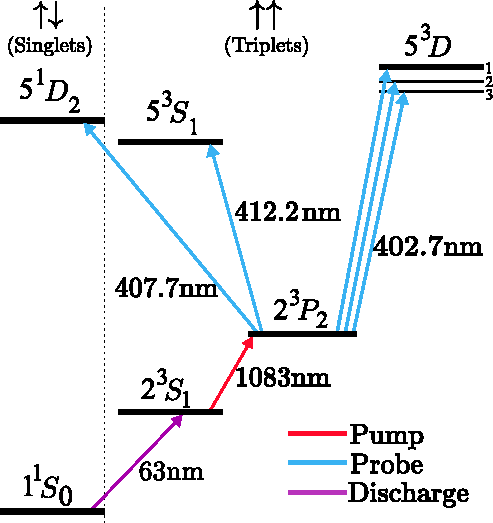
\includegraphics[width=0.45\textwidth]{fig/spectroscopy/level-diagram-tight-latex-pdf.pdf}
      \caption{Energy level diagram for the helium atom.
	The transitions measured in this work (blue) are driven by a tunable laser referred to in the text as the \emph{probe beam}.
	A laser tuned to the $2\triplet S_1-2\triplet P_2$ transition (red, referred to as \emph{pump beam}) populates the lower state of the target transitions.
	 The doubly forbidden $1^{1\!}S_0 - 2^{3\!}S_1$ transition is excited in a high voltage discharge source.
	Transitions across the dotted line are \emph{forbidden} by the $\Delta S=0$ selection rule.
	Level splittings are not to scale.}
      \label{fig:lvl_diag}
  \end{figure}

  A concurrent issue is the so-called `proton radius puzzle': Determinations of the proton charge radius from Lamb shift measurements in muonic and electronic hydrogen \cite{Pohl10, Bezginov19}, electron-hydrogen scattering experiments \cite{Beyer17,Xiong19}, and isotope shifts in light muonic atoms \cite{Kalinowski19,Pohl16} disagree significantly with both the CODATA recommended value and with other recent experiments \cite{Fleurbaey18}.
	 Helium is a promising candidate to provide insight into this unresolved issue because its simple structure is tractable to QED calculations.
	Ongoing theoretical work \cite{Pachucki15,Pachucki17,Pachucki11,Pachucki10,Morton12,Morton06,Patkos16,Patkos17} and recent high-precision measurements \cite{Rooij11,Notermans14,Notermans16,Rengelink18} find a $4\sigma$ discrepancy between the difference $\delta = r^2(^3\textrm{He}) - r^2(^4\textrm{He})$ of squared nuclear charge radii obtained from the isotope shifts of the $\MetastableState - \PStateManifold$ and ${2^{1\!}S_{0}} - \MetastableState$ transitions \cite{Pachucki15,Patkos17}.
	The completed calculation of QED effects to order $\alpha^7$ will allow determination of the absolute nuclear charge radii accurate to better than 1\% \cite{Pachucki17}.
	Along with these $\alpha^7$ contributions, measurement of the $2\triplet P-2\triplet S$ spacing to within 1.4kHz would allow a determination of the nuclear charge radius to below 0.1\% accuracy, better than expected from the muonic helium Lamb shift \cite{Wienczek19}.
	 

  Notable among recent studies of helium's structure are the measurements of \emph{forbidden} transitions between the singlet and triplet manifolds.
	Such transitions are made possible in reality due to relativistic effects and are extremely narrow, therefore precise measurements of their spectral features can provide stringent tests of QED \cite{Lach01}.
	The present work complements existing measurements of forbidden lines in helium at 1557nm \cite{Rooij11,Rengelink18}, 887nm \cite{Notermans14}, and 427nm \cite{Thomas20}.

  In this work, we report on frequency measurements of the transitions from the $2^3P_2$ state to five states in the $n=5$ manifold of $^4$He, illustrated in Fig.
	\ref{fig:lvl_diag}.
	
  Our results improve on the precision of past measurements \cite{Martin60} by at least an order of magnitude.
  We resolve the fine structure splitting of the $\PStateManifold_2 - 5\triplet D$ transition.
	As far as we can ascertain, our work includes the first observation of the spin-forbidden $2^3P_2 - 5^1D_2$ transition in helium, whose transition rate is four orders of magnitude smaller than the other transitions reported here.

  

\section{Experiment}

% Sequence
We performed our measurements by disrupting a laser cooling stage in the production of a Bose-Einstein condensate (BEC) of $^{4}\textrm{He}$ atoms.
	Our experimental sequence begins with $\sim10^8$ atoms in the metastable $2\triplet S_1$ state, cooled to  $\sim1 \textrm{mK}$ in a magneto-optical trap.
	Throughout the sequence, all laser cooling light is tuned to the $2\triplet S_1 - 2\triplet P_2$ transition at 1083.331nm \cite{Shin16}.
	The light is then switched off, leaving only the $m_J=1$ atoms in a magnetic trap generated by field coils in a BiQUIC configuration \cite{Dall07}.
	Next, during a Doppler cooling stage, we illuminated the atoms with $\sim$30$\mu$W$/m^2$ of $\sigma^+$ polarized cooling light in an approximately uniform magnetic field set by the high bias of the BiQUIC coils, further cooling the atoms to $\sim200\mu \textrm{K}$.
	Finally, we applied forced evaporative cooling by RF radiation, cooling the sample below the critical temperature to form a BEC.
	Each iteration of this procedure produced a BEC of $\sim 5\times10^5$ atoms in a cigar-shaped harmonic trap with trapping frequencies $\omega = 2\pi (425,425,45)$ Hz.
	

% Detection
At the end of the experimental sequence the atoms are in the metastable $2^3S_1(m_J=1)$ state, which has a lifetime of $7870$ seconds \cite{Hodgman09}.
	The metastable state is 19.8eV above the true ground state, and this large internal energy enables single-atom detection by a multi-channel plate and delay-line detector stack \cite{Manning10}, located $\sim$850mm below the trap.
	The detector has a quantum efficiency of $\sim 8\%$ and saturates at high atom fluxes, precluding accurate number measurements by simply dropping a BEC on the detector.
	Instead, we used a \emph{pulsed atom laser}, wherein broadband radio-frequency pulses transfer $\sim$2\% of the trap population {at a time} to the untrapped $2\triplet S_1(m_J=0)$ state \cite{Manning10,Henson18}.
	The resulting coherent matter-wave pulse{s} fall onto the detector, {depleting the entire trapped population after $\sim$200 pulses over 2 seconds.
	This allows}  the atom number and temperature to be accurately determined without saturating the detector.
	Each iteration of the BEC preparation sequence followed by detection is referred to as a \emph{shot}.
	Our data collection protocol consisted of a cycle of one calibration shot with the probe beam switched off, followed by one measurement shot at each of two magnetic field strengths with the probe beam on.
	

The physical basis of our measurement is the sensitivity of forced evaporative cooling to the initial conditions of the helium atoms.
	The precise effect of photon scattering on the final cloud properties depends on the exact details of the evaporation sequence, and is hard to model exactly.
	Instead, we give a qualitative picture of the role evaporative cooling plays in transforming photon scattering to a measurable change in trap population.
	

During the Doppler cooling stage of BEC creation, the 1083nm cooling beam acts as an optical pump and excites atoms to the $2\triplet P_2(m_J=2)$ state.
	From the $2\triplet P_2$ state they may decay, with a $\sim$97ns lifetime, back to the trapped metastable state or absorb photons from the probe beam and become excited again to the target state.
	Doubly-excited atoms may decay back to the trapped $m_J=+1$ state of the $2\triplet S_1$ level, in which case the photon absorption and emission events add heat to the cloud by imparting a nonzero average impulse to the atoms.
	An initially hotter cloud therefore reduces the efficiency of evaporative cooling, resulting in a higher atom loss during the process and a lower final number in the trap.
	

Alternatively, atoms may decay to other untrapped magnetic states of the metastable state, or to the true ground state via a spin-flip transition to the singlet manifold.
	Decay to untrapped states reduces the initial atom number and can even impart heat to the cloud as these atoms leave the trap - via scattering with trapped atoms.
	This heating will be much smaller than in the previous case because the scattering rate will be small in such a dilute gas.
	However, reducing the initial trap population also manifests as a reduced final atom number.
	In both cases a photon scattering signal clearly manifests in the reduction of the total trapped final number $N$ relative to the final number $N_c$ in calibration shots.
	We define our signal to be the relative number loss $(N_c-N)/N_c$ to compensate for drift in the trap population over time.

\begin{figure}
  \begin{minipage}[t]{0.6\textwidth}
  \vspace{0pt}
        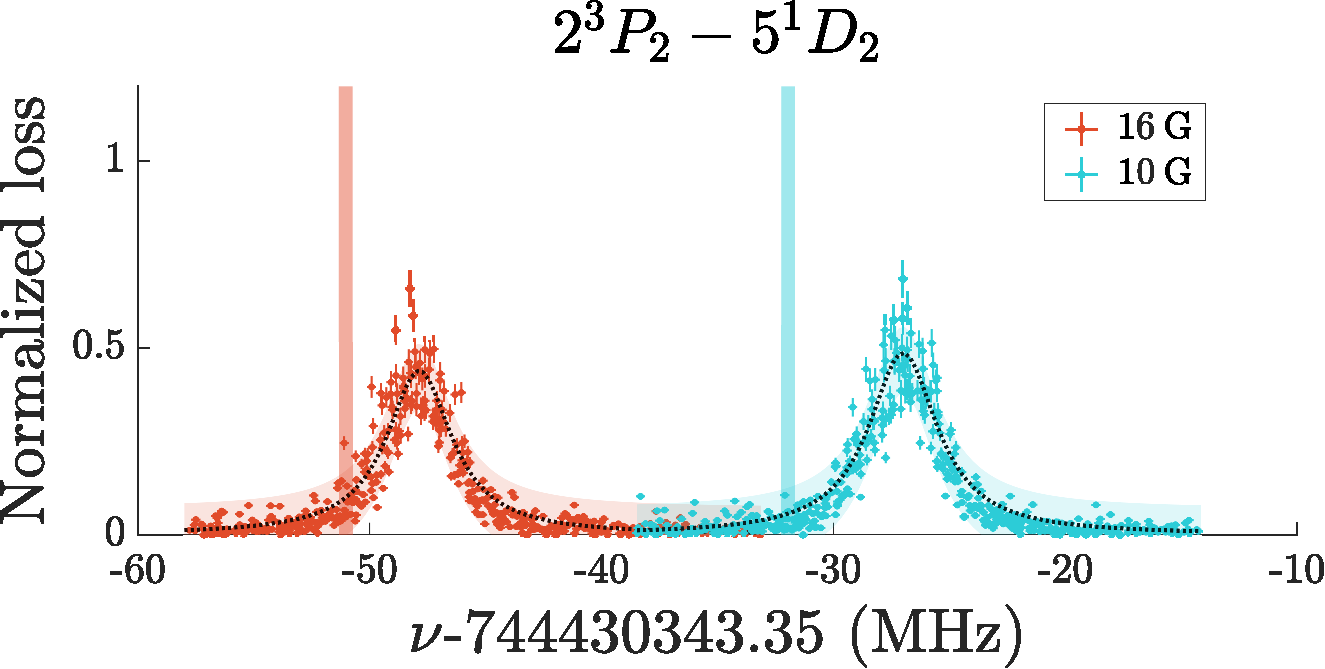
\includegraphics[width=\textwidth]{fig/spectroscopy/ci-plot-51D2-eps-converted-to.pdf}
    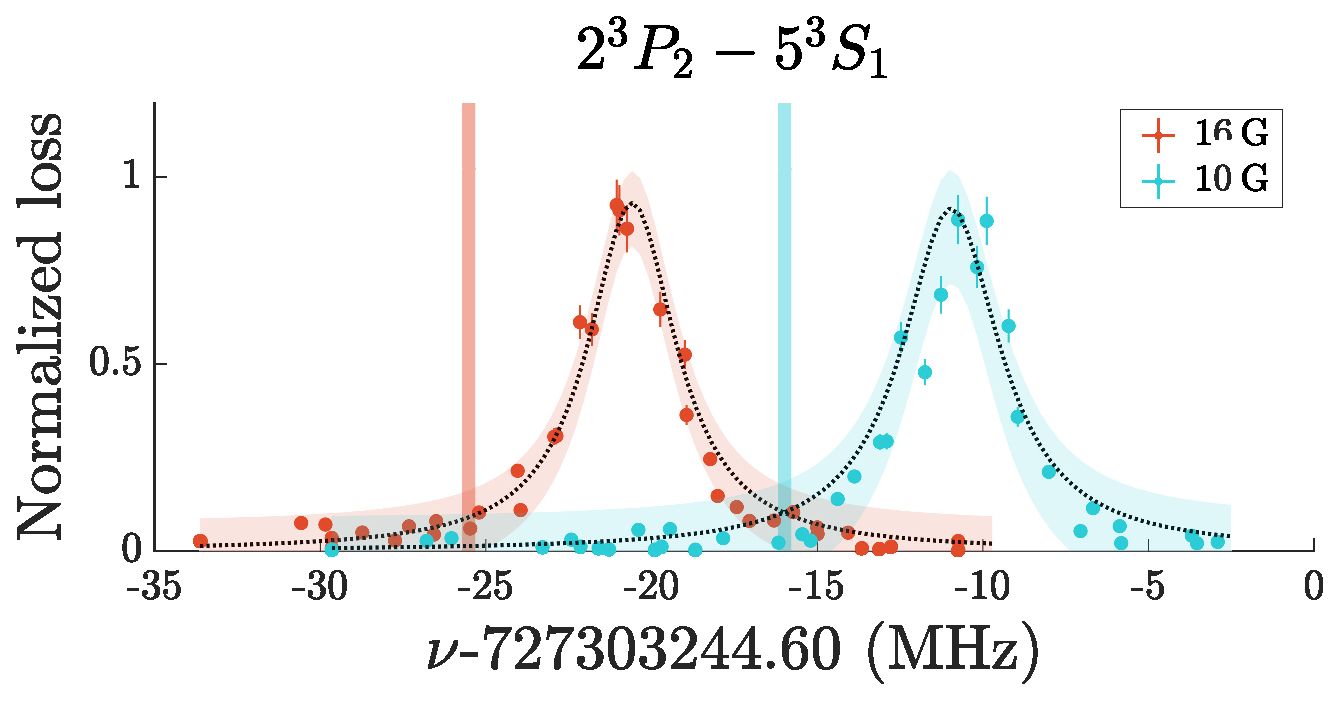
\includegraphics[width=\textwidth]{fig/spectroscopy/ci-plot-53S1}
  \end{minipage}\hfill
  \begin{minipage}[t]{0.38\textwidth}
  \vspace{0pt}
   \caption{Line profile for the spin-forbidden $\PStateManifold_2 -  5^{1\!}D_2$ and the $2\triplet P_2 - 5\triplet S_1$ resonances, showing normalized atom number loss versus probe laser frequency $\nu$, as measured in an {16.8(1)}G (red) and {10.06(7)}G (blue) background field, with Lorentzian fits (black dotted line, with prediction confidence interval shaded).
	Error bars account for detector efficiency and calibration model uncertainty.
	For comparison, theoretical predictions (vertical bars) Zeeman shifted from the predicted zero-field value \cite{Drake07} according to the field calibration, whose uncertainty (shaded width) is dominated by background field measurements.}
    \label{fig:1D_2_line}
  \end{minipage}
\end{figure}


% \begin{figure}
%     \centering
%     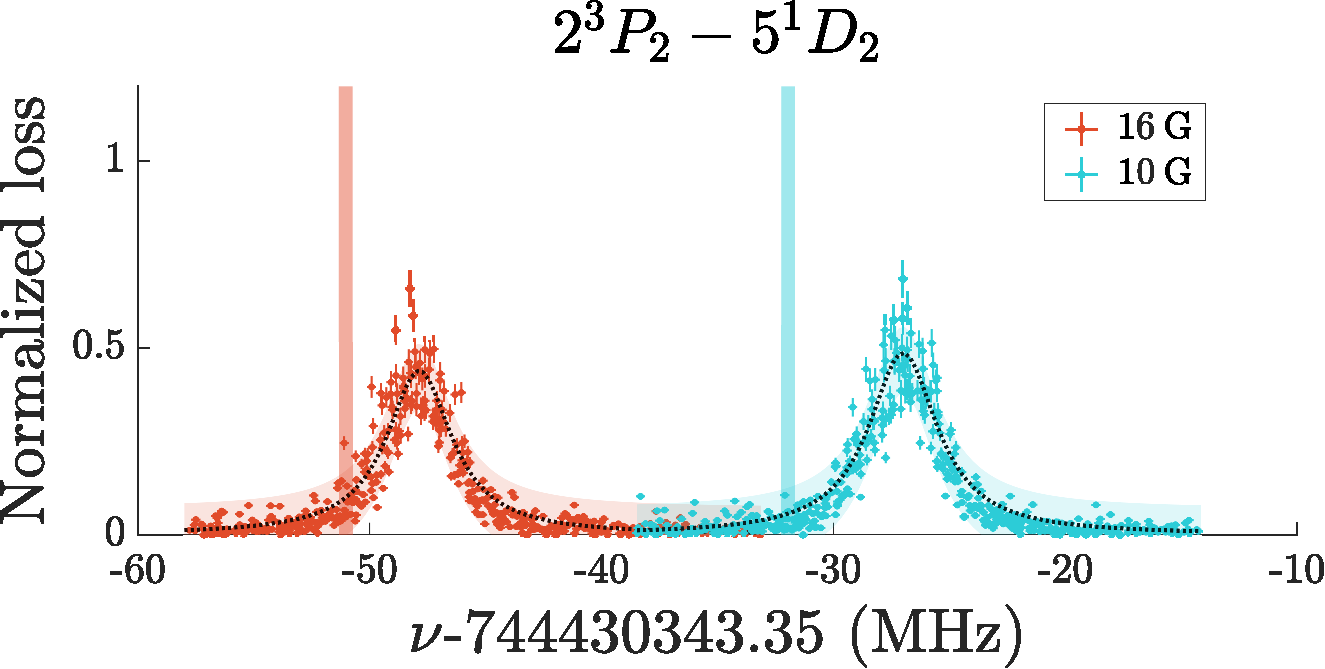
\includegraphics[width=0.66\textwidth]{fig/spectroscopy/ci-plot-51D2-eps-converted-to.pdf}
%     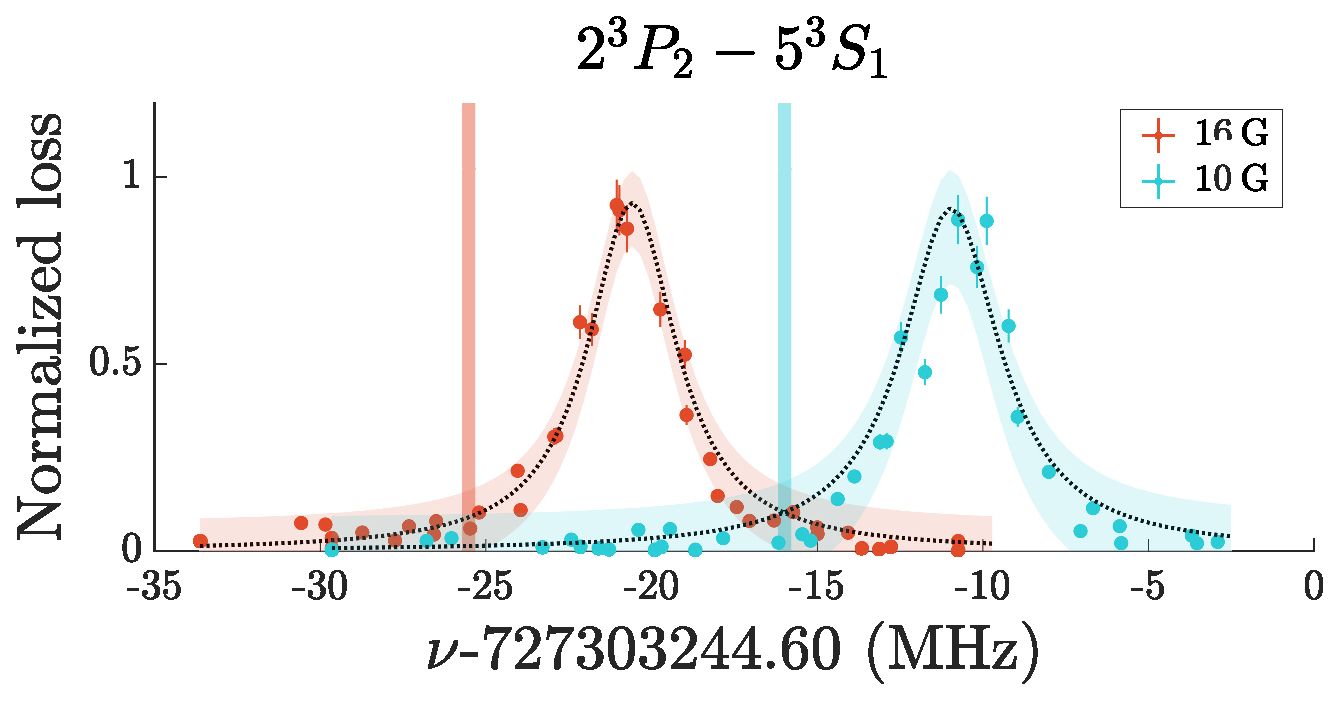
\includegraphics[width=0.66\textwidth]{fig/spectroscopy/ci-plot-53S1}
%     \caption{Line profile for the spin-forbidden $\PStateManifold_2 -  5^{1\!}D_2$ and the $2\triplet P_2 - 5\triplet S_1$ resonances, showing normalized atom number loss versus probe laser frequency $\nu$, as measured in an {16.8(1)}G (red) and {10.06(7)}G (blue) background field, with Lorentzian fits (black dotted line, with prediction confidence interval shaded).
% 	Error bars account for detector efficiency and calibration model uncertainty.
% 	For comparison, theoretical predictions (vertical bars) Zeeman shifted from the predicted zero-field value \cite{Drake07} according to the field calibration, whose uncertainty (shaded width) is dominated by background field measurements.}
%     \label{fig:1D_2_line}
%   \end{figure}


% Laser
To generate the probe beam light, we used 532nm light from a Lighthouse Photonics Sprout module to pump a tunable M-squared SolsTi:S titanium-sapphire laser, tuned near 800nm, and frequency-doubled the output in an M-squared ECD-X module to produce the target wavelengths.
	A sample of the Ti:S output was fibre coupled to a High Finesse WS8 wavemeter.
	A software lock used the wavemeter output to stabilize the laser and to scan the probe beam frequency across the region of interest.
	We calibrated the wavemeter by saturated absorption spectroscopy of cesium in a vapor cell.
	Our frequency reference was the $6S_{1/2}(F=3)-8S_{1/2}(F=3)$ two-photon transition in cesium at $364507238.36(1)$MHz \cite{Wu13}.
	To minimize wavemeter drifts over time, we calibrated the wavemeter daily, observing maximum drifts of order 1MHz over this timescale.
	

We used the first diffracted mode of an acousto-optical modulator (AOM) to control the probe beam power.
	The output of the AOM was fibre coupled to the vacuum insertion optics, where a photodiode provided the input for PID control of the beam power.
	The profile and polarization of the beam were set manually with lenses and waveplates prior to vacuum entry.
	Additional details about the experimental setup can be found in the supplementary materials of Ref.
	\cite{Thomas20}.


To make our measurements of the transition frequencies for the $5\singlet D_2$ and $5\triplet S_1$ states, we illuminated the atoms with the probe light for periods of order 100 ms during the Doppler cooling stage.
	The exact duration differed for each line to obtain a good SNR without saturating the atom loss.
	The light was $\sigma^-$ polarized to drive transitions to the $m_J=1$ states of the upper levels.
	For the forbidden $5\singlet D_2$ transition the beam was focused on the atom cloud with a waist of approximately $100\mu$m and a peak intensity of order $5\times 10^3$ W/m$^2$.
	For all other measurements the beam was collimated with a peak intensity of order $ 5$ W/m$^2$.
	We took measurements at two points in the Doppler cooling stage with a bias field strengths of {16.5(3)} and {10.2(3)} Gauss, which we calibrated independently by RF spectroscopy.
	For each field strength we obtained the atom loss (with respect to calibration shots) versus probe laser frequency.
	After correcting for the measured AOM and vapor cell shifts, we fit the measured response with a Lorentzian function, as shown in Figs.
	\ref{fig:1D_2_line} and \ref{fig:5_3S_1}.
	{The transduction from photon scattering to atom loss via evaporative cooling is complicated and not linear.
	However, we found that fits using a nonlinear function of the Lorentzian lineshape differed from the simple Lorentzian fit by substantially less than the statistical uncertainty.}

We correct for the linear Zeeman shift to estimate the field-free transition frequencies with sub-MHz statistical uncertainty.
	This determines the $2\triplet P_2-5\singlet D_2$ and $2\triplet P_2-5\triplet S_1$ transition energies to be 3MHz and 5MHz larger, respectively, than the predictions presented in \cite{Drake07}.
	However, the absolute accuracy of these measurements is limited by our instrumentation.
	Our results (Tab.
	\ref{tab:results}) are consistent with current predictions \cite{Drake07} within $2\sigma$ after accounting for all systematic uncertainties (Tab.
	\ref{tab:errors}).

% \begin{figure}
%     \centering
%     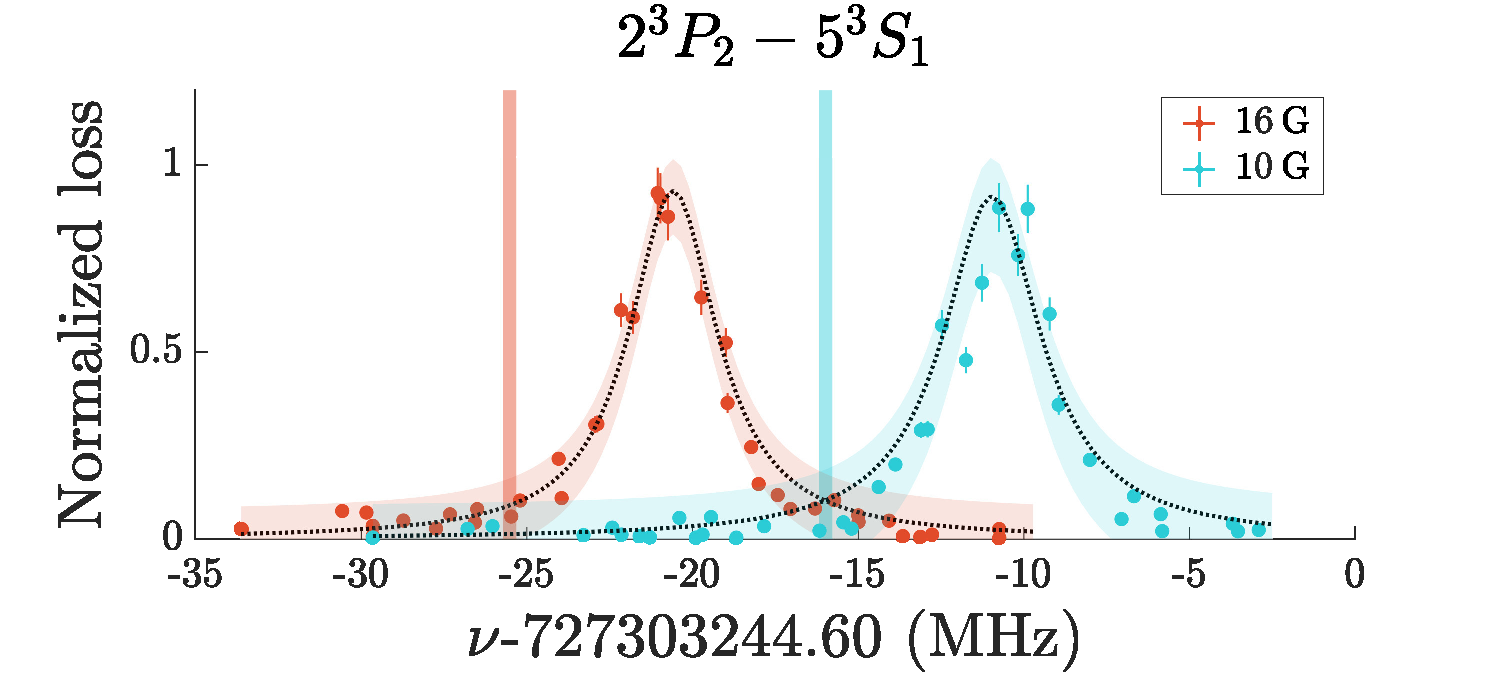
\includegraphics[width=0.48\textwidth]{fig/spectroscopy/ci-plot-53S1-eps-converted-to.pdf}
%     \caption{Measured atom loss versus laser frequency for  resonance in comparison to Zeeman-shifted predictions \cite{Drake07}, shown as for Fig.
% 	\ref{fig:1D_2_line}}
%     \label{fig:5_3S_1}
% \end{figure}

\section{5$\triplet$D fine structure}

Unlike the $5\singlet D_2$ and $5\triplet S_1$ levels, the $5\triplet D$ manifold splits into fine structure sublevels, leading to multiple absorption peaks and requiring a more involved analysis.
	We drove transitions to the $5\triplet D_J, J\in\{1,2,3\}$ levels with a combination of $\pi$ and $\sigma^-$ polarized light (in the atomic frame) and obtained four peaks, as shown in Fig.
	\ref{fig:combined_5D_lines}.
	The saturated peak near -300MHz (relative to the predicted $2\triplet P_2 - 5\triplet D_1$ interval) is in fact two peaks corresponding to the $5\triplet D_2(m_J=1)$ and $5\triplet D_3(m_J=2)$ states, which are separated by less than their linewidth.
	This illustrates a shortcoming of our technique, namely the limited dynamic range.
	For measurements of single peaks this is not an issue as the total irradiated energy can be adjusted to obtain a good signal-to-noise ratio without completely depleting the BEC.
	In this case, however, there is a trade-off between keeping the small peaks above the noise floor and preventing the superposed peaks from saturating.
	This limitation could be eased with a larger initial condensate because the dynamic range is essentially limited by the atom loss.

The Zeeman shift of the $J=2$ and $J=3$ levels is comparable to the interval between them, and so the mixing of levels means the correction is no longer proportional to $B$.
	Instead, we solve the eigenvalue optimization problem 
%
\begin{equation}
\textrm{min}_{E_{\textrm{fs}}} \sum_{J,m_J} \left(\nu_{{J,m_J}}^{\textrm{{pred}}}(E_{\textrm{fs}},B) - \nu_{{J,m_J,B}}^{\textrm{{obs}}}\right)^2,
\label{eqn:opt-problem}
\end{equation}
%
which minimizes the squared error between observed and predicted transition frequencies ($\nu^{\textrm{{obs}}}$ and $\nu^{{\textrm{pred}}}$ respectively), summed over all relevant $|J,m_J\rangle$ states and magnetic field strengths $B$.
	The optimized variable $E_{\textrm{fs}}=(E_1,E_2,E_3)$ is the bare fine-structure splitting of the $5\triplet D$ levels.
	In the argument below we assume only the formalism of atomic structure theory and the data from our experiment.
	To determine the bare $5\triplet D$ transition energies from our data, consider the Hamiltonian
%
\begin{equation}
    \hat{H}(B) = \hat{H}_{\textrm{fs}} - B\hat{\mu}_z,
    \label{eqn:hamiltonian}
\end{equation}
%

\begin{figure}
	\centering
	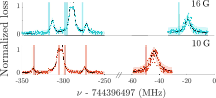
\includegraphics[width=\textwidth]{fig/spectroscopy/ci-plot-53D}
   \caption{Line profiles for the $\PStateManifold_2 -  5^{3\!}D$ transitions, shown as for Figs.
	\ref{fig:1D_2_line} and \ref{fig:5_3S_1}.
	The normalized loss is shown versus probe laser frequency for the two different field strengths with a common horizontal scale.
	Theory lines indicate predictions from \cite{Drake07} after applying the relevant Zeeman shift.
	N.B.	the scale break here and in Fig.	\ref{fig:fitting_3D} coincide.}
    \label{fig:combined_5D_lines}
\end{figure}

% \begin{figure}
%   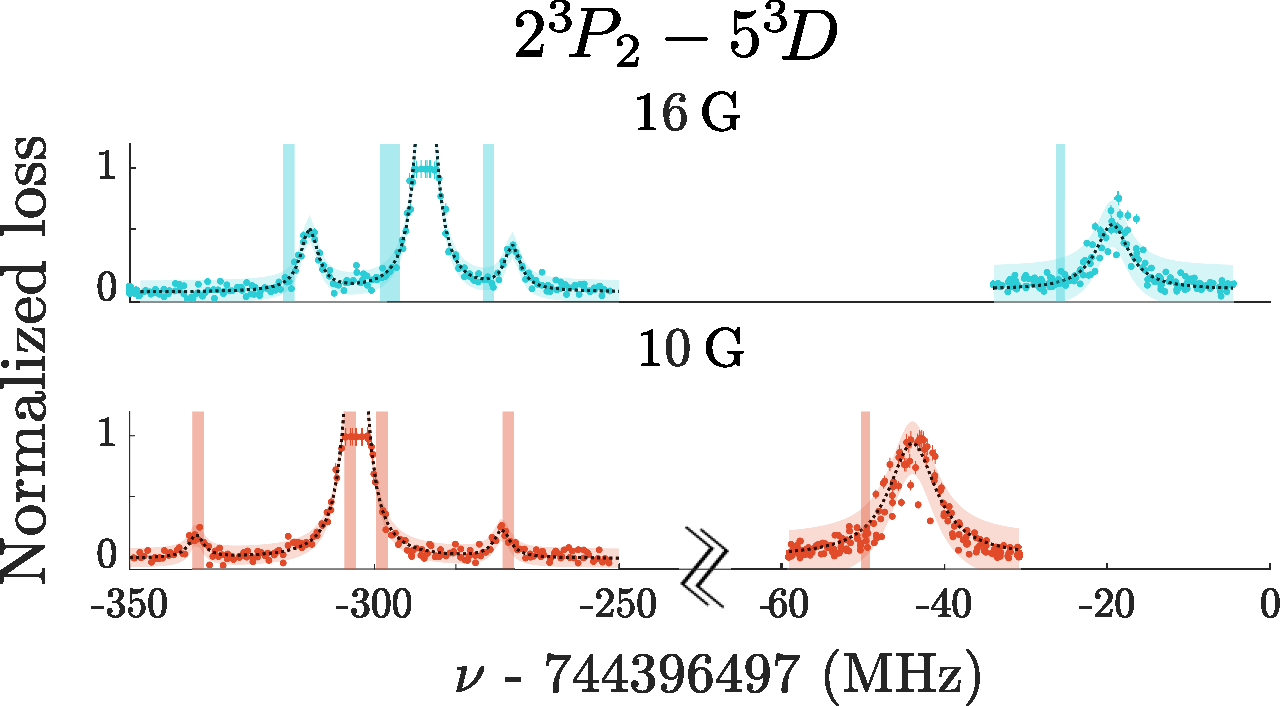
\includegraphics[width=0.5\textwidth]{fig/spectroscopy/ci-plot-53D-eps-converted-to.pdf}
%   \caption{Line profiles for the $\PStateManifold_2 -  5^{3\!}D$ transitions, shown as for Figs.
% 	\ref{fig:1D_2_line} and \ref{fig:5_3S_1}.
% 	The normalized loss is shown versus probe laser frequency for the two different field strengths with a common horizontal scale.
% 	Theory lines indicate predictions from \cite{Drake07} after applying the relevant Zeeman shift.
% 	N.B.	the scale break here and in Fig.	\ref{fig:fitting_3D} coincide.}
%   \label{fig:combined_5D_lines}
% \end{figure}

%
where $\hat{\mu}_z = \mu_B(\hat{L}_z + g_s \hat{S}_z)/\hbar$ is the coupling of the orbital and spin angular momenta of the electron with a magnetic field of strength B pointing in the $z$-direction, $\mu_B$ is the Bohr magneton and $g_s$ is the electron spin $g$-factor.
	The fine structure Hamiltonian $\hat{H}_{\textrm{fs}}$ is diagonal in the $|LSJ m_J\rangle$ basis with eigenvalues $E_{\textrm{fs}}$,
%
\begin{equation}
  \hat{H}_{\textrm{fs}}|LSJm_J\rangle = E_{\textrm{fs},LSJ}|LSJm_J\rangle,
\end{equation}
%
which are degenerate for all $m_J$ with fixed $J$.
	The magnetic moment $\hat{\mu}_z$ couples states of different $J$, and is instead diagonal in the $|L m_L S m_S\rangle$ basis.
	In the $|LSJ m_J\rangle$ basis the matrix elements of $\hat{H}(B)$ are, with abbreviated notation,
%
\begin{equation}
\begin{aligned}
H_{J',J} =& \langle J'|\hat{H}|J \rangle\\
  =& E_{\textrm{fs},J} - B \frac{\mu_B}{\hbar} \sum_{m_L} (2m_J - m_L)C_{J,'m_L}C_{J,m_L},\\
\end{aligned}
\end{equation}
%
where $C_{J,m_L} = \langle LSJ m_J|L m_L S m_S\rangle$ is shorthand for the Clebsch-Gordan coefficients.
	For $B>0$, the contribution of $\hat{\mu}_z$ breaks the degeneracy of $\hat{H}_{\textrm{fs}}$, giving rise to the Zeeman shift.
	
%
%

\begin{table*}
\centering
  % \begin{tabular}{c c c c c c c c c c c}
  %     \hline\hline
  %     Transition                        & &  $f_\textrm{exp}$ & &  $f_\textrm{theory}$ & Ref.
		% &  $f_\textrm{exp}-f_\textrm{theory}$      & &  $\textrm{FWHM}_{\textrm{exp}}$  & &  $\textrm{FWHM}_{{\textrm{pred}}}$ \\
  %     \hline
  %       $2\triplet P_2 - 5^3\mathrm{S}_1$ & &  {727,303,248(3)} & &  727,303,244.6(4)   & \cite{Drake07} &  {3(3)}    & &  3.4(5)  & &  1.5\\ % A = 
  %       $2\triplet P_2 - 5^3\mathrm{D}_1$ & &  {744,396,496(7)} & &  744,396,511.1(7)   & \cite{Yerokhin20} &  {-16(7)}    & &  5.8(6)  & &  2.6\\
  %       $2\triplet P_2 - 5^3\mathrm{D}_2$ & &  {744,396,220(7)} & &  744,396,227.6(7)   & \cite{Yerokhin20} &  {-8(7)}    & &  4.2(5)  & &  2.6\\
  %       $2\triplet P_2 - 5^3\mathrm{D}_3$ & &  {744,396,194(7)} & &  744,396,208.3(7)   & \cite{Yerokhin20} &  {-14(7)}    & &  4.0(1)  & &  2.6\\
  %       $2\triplet P_2 - 5^1\mathrm{D}_2$ & &  {744,430,343(7)} & &  744,430,343.1(7)   & \cite{Yerokhin20} &  {0(7)}    & &  3.2(1)  & &  2.2\\  % 744430344
  %     \hline\hline
  %   \end{tabular}

    \begin{tabular}{c c c c c c c c c c c}
      \hline\hline
      Transition                        &  $f_\textrm{exp}$ &  $f_\textrm{theory}$ & Diff.
		  &  $\textrm{FWHM}_{\textrm{exp}}$  &  $\textrm{FWHM}_{{\textrm{pred}}}$ \\
      \hline
        $2\triplet P_2 - 5^3\mathrm{S}_1$ &  {727,303,248(3)} &   727,303,244.6(4)   &  {3(3)}      &  3.4(5)  &  1.5\\ % A = 
        $2\triplet P_2 - 5^3\mathrm{D}_1$ &  {744,396,496(7)} &   744,396,511.1(7)   &  {-16(7)}     &  5.8(6)  &  2.6\\
        $2\triplet P_2 - 5^3\mathrm{D}_2$ &  {744,396,220(7)} &   744,396,227.6(7)   &  {-8(7)}      &  4.2(5)  &  2.6\\
        $2\triplet P_2 - 5^3\mathrm{D}_3$ &  {744,396,194(7)} &   744,396,208.3(7)   &  {-14(7)}     &  4.0(1)  &  2.6\\
        $2\triplet P_2 - 5^1\mathrm{D}_2$ &  {744,430,343(7)} &   744,430,343.1(7)   &  {0(7)}      &  3.2(1)  &  2.2\\  % 744430344
      \hline\hline
    \end{tabular}
\caption{Summary of results for each transition.
	After correcting for the AOM and vapor cell shifts we extract the centre frequencies from Lorentzian fits with statistical error at the $10\textrm{kHz}$ level.
	We obtain the field-free energies after correcting for Zeeman shifts, shown with theoretical predictions in the row below.
	We show the difference between our measurements and theoretical predictions for direct comparison.
	Observed full width at half maximum line widths (FWHM) of the Lorentzian fit to each line are shown in comparison to predicted linewidths as given in \cite{Drake07}.
	$f_\textrm{theory}$ for the $2\triplet P_2 - 5^3\mathrm{S}_1$ line comes from \cite{Drake07}, all others from \cite{Yerokhin20}
	All values are in MHz with uncertainty in the final digit in parentheses.}
  \label{tab:results}
\end{table*}
The solution of Eqn.
	\ref{eqn:opt-problem} is illustrated in Fig.
	\ref{fig:fitting_3D}.
	If we define the energies $E_{\textrm{fs}}$ relative to the $2\triplet P_2(m_J=2)$ state, then we can read the predicted transition frequencies directly from the eigenvalues of $\hat{H}$ via $\nu_{J,m_J}^{\textrm{pred}}=E_{J,mJ}(B)/h$, where $h$ is Planck's constant.
	The observed frequencies $\nu_{J,m_J,B}^{\textrm{obs}}$ used in this procedure exclude the saturated peaks because their centre frequencies cannot be determined accurately.
	The triple $E_{\textrm{fs}}$ which minimizes the cost function (Eqn.
	\ref{eqn:opt-problem}) corresponds to the $2\triplet P_2 - 5\triplet D_J$ intervals at $B=0$, as listed in Tab.
	\ref{tab:results}.
	Again, the difference in our determination of the field-free splitting is consistent within 2$\sigma$ predictions in \cite{Drake07} after accounting for systematic effects (Tab.
	\ref{tab:errors}).
	


% \usepackage{floatrow}



% \begin{figure}
% \floatbox[{\capbeside\thisfloatsetup{capbesideposition={left,top},capbesidewidth=4cm}}]{figure}[\FBwidth]
% {\caption{A test figure with its caption side by side}\label{fig:test}}
% {\includegraphics[width=5cm]{name}}
% \end{figure}

% \begin{figure}
% \floatbox[{\capbeside\thisfloatsetup{capbesideposition={right,top},capbesidewidth=4cm}}]{figure}[\FBwidth]
% {\caption{A test figure with its caption side by side}\label{fig:test}}
% {\includegraphics[width=5cm]{name}}
% \end{figure}


\begin{figure}
\centering
	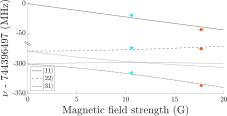
\includegraphics[width=0.8\textwidth]{fig/spectroscopy/fitting-lines}
	\caption{Determining the $5\triplet D$ fine-structure splitting.
	The values for the $|J,m_J\rangle=5\triplet D_J(m_J)$ levels (grey lines) at $B=0$ are fixed by solving the optimization problem (Eqn.
	\ref{eqn:opt-problem}), constrained by the fitted peak centres (filled circles).
	The saturated peaks are not used to constrain the levels, but are shown with hollow circles and the corresponding frequencies predicted by our method are shown in dotted lines.}
    \label{fig:fitting_3D}
\end{figure}


% \begin{figure}
% 	\begin{minipage}[t]{0.38\textwidth}
% 			\vspace{0pt}
% 			\caption{Determining the $5\triplet D$ fine-structure splitting.
% 	The values for the $|J,m_J\rangle=5\triplet D_J(m_J)$ levels (grey lines) at $B=0$ are fixed by solving the optimization problem (Eqn.
% 	\ref{eqn:opt-problem}), constrained by the fitted peak centres (filled circles).
% 	The saturated peaks are not used to constrain the levels, but are shown with hollow circles and the corresponding frequencies predicted by our method are shown in dotted lines.}
%     \label{fig:fitting_3D}
% 	\end{minipage}\hfill
% 	\begin{minipage}[t]{0.6\textwidth}
% 		\vspace{0pt}
% 		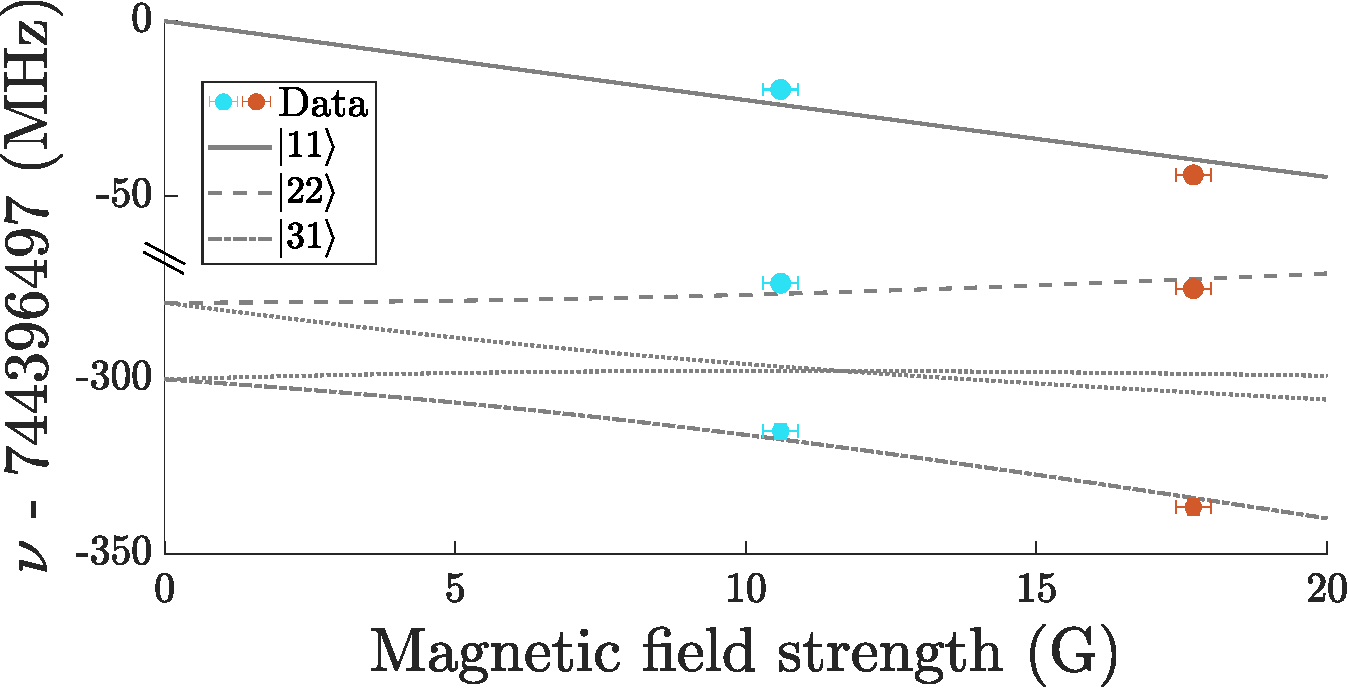
\includegraphics[width=\textwidth]{fig/spectroscopy/fitting-lines-eps-converted-to.pdf}
% 	\end{minipage}

% \end{figure}

% \begin{figure}
%     \centering
%     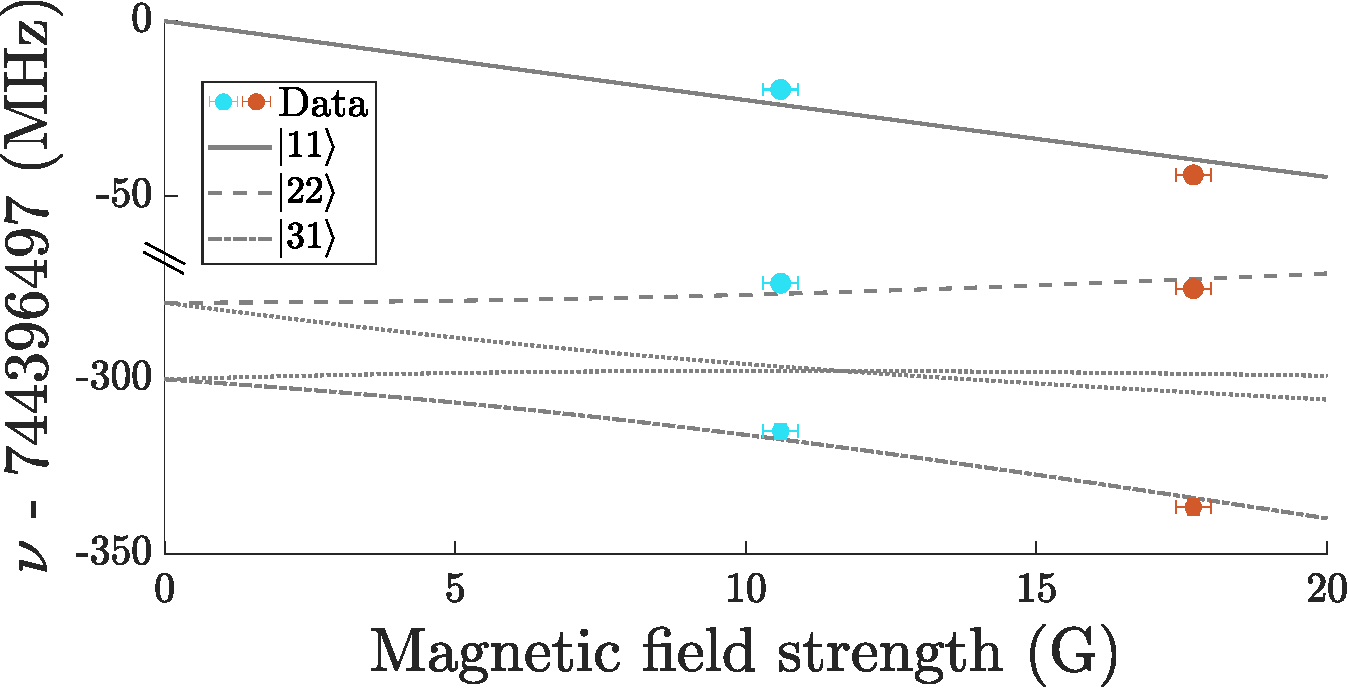
\includegraphics[width=0.48\textwidth]{fig/spectroscopy/fitting-lines-eps-converted-to.pdf}
%     \caption{Determining the $5\triplet D$ fine-structure splitting.
% 	The values for the $|J,m_J\rangle=5\triplet D_J(m_J)$ levels (grey lines) at $B=0$ are fixed by solving the optimization problem (Eqn.
% 	\ref{eqn:opt-problem}), constrained by the fitted peak centres (filled circles).
% 	The saturated peaks are not used to constrain the levels, but are shown with hollow circles and the corresponding frequencies predicted by our method are shown in dotted lines.}
%     \label{fig:fitting_3D}
% \end{figure}

\section{Shifts, broadening, and errors}




\begin{table}
\centering
  \begin{tabular}{c c c}
      \hline\hline
          Source & Shift & Broadening  \\
      \hline
          Wavemeter ($5\triplet S_1$)& 0(1.3) & - \\
          Wavemeter (all other lines)& 0(6.7) & - \\
          Pump lock & - & 4$\times10^{-2}$ \\
          Pump AOM & - & 0.3 \\
          Probe lock & - & 0.3\\
          Probe AOM & -189 & 1$\times10^{-6}$\\
          Zeeman & Variable & Variable \\
          Recoil & - & 1.4$\times 10^{-3}$ \\ % assume angle accurate to 1deg
          Doppler & - & 2.7(4) \\
          Interference effects & 0.5 & - \\ 
          Cs cell & -1.9 & 0.4 \\
          \textbf{Total} ($5\triplet S_1$ level) & -190.9(1.7)+ZS& 2.2\\
          \textbf{Total} (all other levels) & -190.9(6.7)+ZS& 2.2\\
      \hline\hline
  \end{tabular}
\caption{Error budget for the determination of the peak centre frequencies.
	 The master laser for our pump beam is described in \cite{Shin16}.
	AOM stabilities were checked with an RF spectrum analyser.
	See \cite{Thomas20} for measurement of the Cesium cell shift and probe beam lock drift.
	The shift and uncertainty from the Zeeman shift (ZS) varies between the lines, so these contributions are omitted from the total.
	All values are in MHz.}
  \label{tab:errors}
  
\end{table}


% summarize results

The results of our measurements are reported in Tab.
	\ref{tab:results} and are consistent with theoretical predictions \cite{Morton06} within $2.1\sigma$ or less.
	The accuracy of our determinations of the field-free transition energies is limited by the absolute accuracy of the wavemeter.
	High Finesse specifies \cite{HighFinesseDoc} a 3$\sigma$ accuracy of 2MHz within 2nm of a calibration line (as in the transition to the $5\triplet S_1$ state), and 10MHz for all other lines measured in this work.
	Because we use the wavemeter to lock the seed light for the doubler, the uncertainty is doubled in determinations of the absolute probe frequency.
	We adopt the corresponding 1$\sigma$ accuracy in order to be consistent with other terms in our error budget, as displayed in Table \ref{tab:errors}.
	We note that this specification does not depend on the specific difference between the calibration and measured wavelengths, and may vary due to nonlinear dispersion of the wavemeter optics.
	Without an independent calibration we cannot rigorously constrain this source of error, which would be overcome with the instrumental improvements discussed below.
	As such, we state the 1-sigma errors determined in this way with the caveat that they may be slightly underestimated.
	Still, all measured frequencies are consistent with predictions to within 2.1$\sigma$.
	Finally, we note that the the $5\triplet S_1$ transition line is 1.9nm away from the calibration line, and as such the 2MHz uncertainty may again be a slight underestimate.

The linewidth of the pump and probe laser sources are 40kHz \cite{Shin16} and 200kHz \cite{Thomas20}, respectively.
	The laser lock error has a standard deviation of $100$kHz.
	The additional contribution from the pump and probe AOMs are 300kHz and 1Hz, respectively, as determined with an RF spectrum analyser.
	

{We calibrated our magnetic field by measuring the change in number of atoms which were detected in response to applied RF radiation.
The number $n_\delta(\nu)$ of detections probes the population of trapped atoms $n_\text{T}(B)$ subject to a magnetic field strength $B$ through the relation $2 \mu_B B = h \nu$.
	
As shown in Fig.
	\ref{fig:RF_spec}, $n_\text{D}(B)$ follows a Bose-Einstein distribution with a chemical potential $g \mu_B B_0$, where $B_0$ is the bias in the magnetic field strength and $g\approx2$ is the g-factor of the $2\triplet S_1$ state.
The Bose-Einstein fit provides a model for $n_\text{T}(B)$ and an estimate of the temperature of the cloud.
	The temperature determination of $\sim130(20)\mu K$ implies Doppler broadenings of 100(10) kHz and 2.6(3) MHz for the pump and probe transitions, respectively.

The optical absorption profile near the 1083nm pump transition can be calculated by convolving $n_\text{T}(B)$ with Zeeman-shifted absorption profile of the 1083nm transition, which is a Lorentzian $\mathcal{L}_\text{abs}(f,B)$ with a 1.6 MHz FWHM \cite{Drake07}.
The pumping rate at a given field strength is given by the convolution of $\mathcal{L}_\text{abs}(f,B)$ with the pump laser line $\mathcal{L}_\text{L}(f)$.
Hence, we calculate the range of magnetic field strengths $B$ at which atoms are pumped to the $2\triplet P_2$ state, which are concentrated at field strengths of 10.2(3) G and 16.5(3) G for the two measurement stages.
	
The Zeeman shift of the $2\triplet P_2 - 5L, L\neq D$ transitions by is given by $\Delta E = \mu B (g_e m_e-g_g m_g)$, whose error is obtained by standard propagation of uncertainties.
	
For the $5\triplet D$ states, we varied the input magnetic field constraints within the range of experimental uncertainty ($0.3$G) to estimate the uncertainty in the iterative method described above.}


\begin{figure}
	\centering
  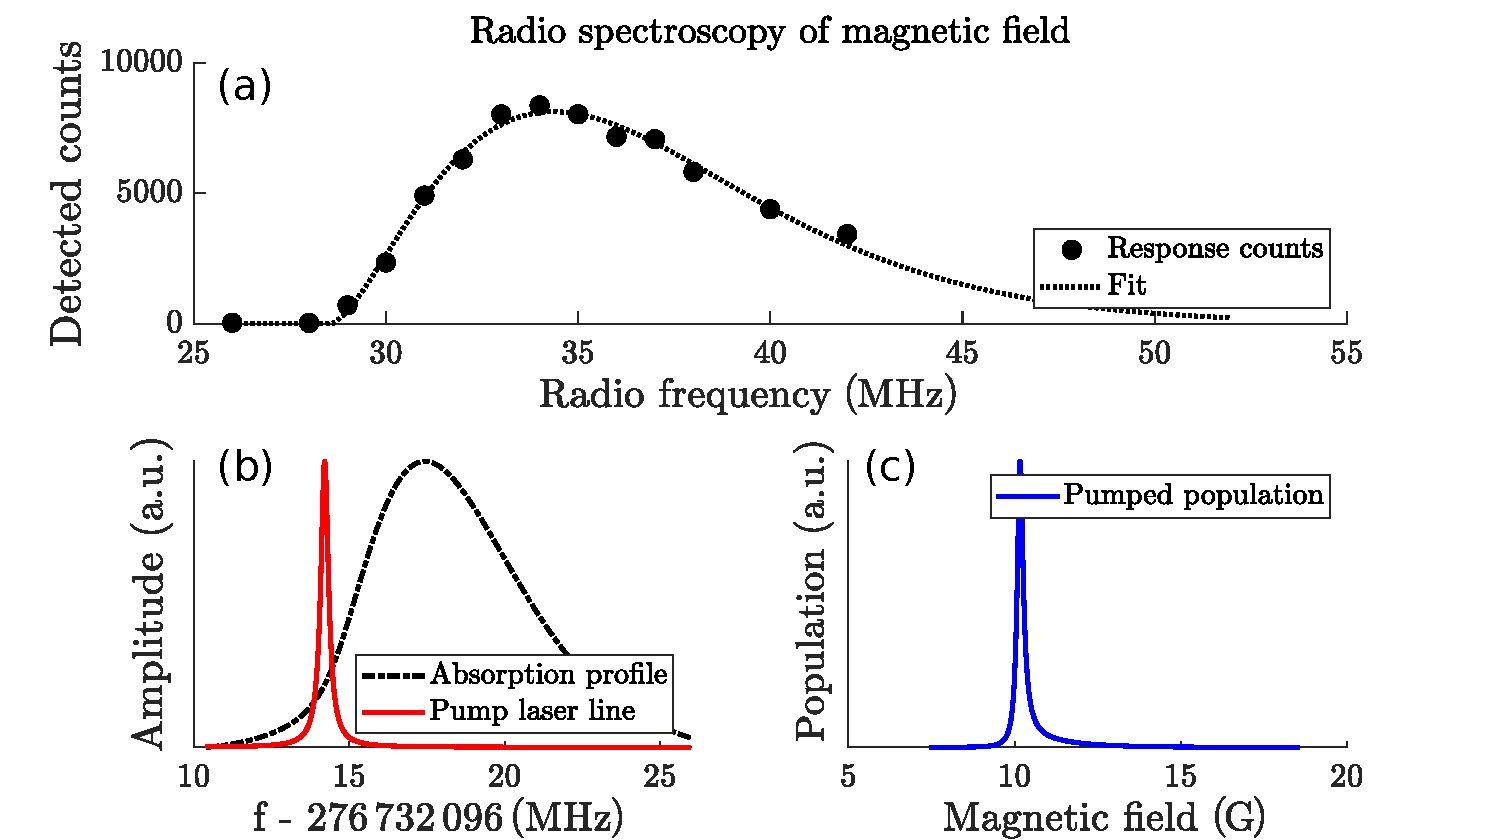
\includegraphics[width=0.9\textwidth]{fig/spectroscopy/rf_spec_subfig-eps-converted-to.pdf}
  \caption{Determination of magnetic field for Zeeman shift correction.
	The number $n_\text{D}$ of atoms detected after probing the trap with 300ms of RF radiation is shown in (a) versus the frequency of the applied radiation.
	Each point is an average of three shots.
	A Bose-Einstein fit models the population density $n_\text{T}$ of the $2\triplet S_1$ state at a given field strength.
	In (b) the calculated absorption profile of the gas in the vicinity of the 1083nm pump transition is shown, along with the spectral profile of the pump laser.
	The pump laser selectively excites atoms with a certain Zeeman splitting, leading to a population of atoms in the $2\triplet P_2$ state (c) that is concentrated around a specific magnetic field strength.
	The resulting Zeeman broadening is dominated by the probe beam linewidth.}
  \label{fig:RF_spec}
\end{figure}


% \begin{figure}
% 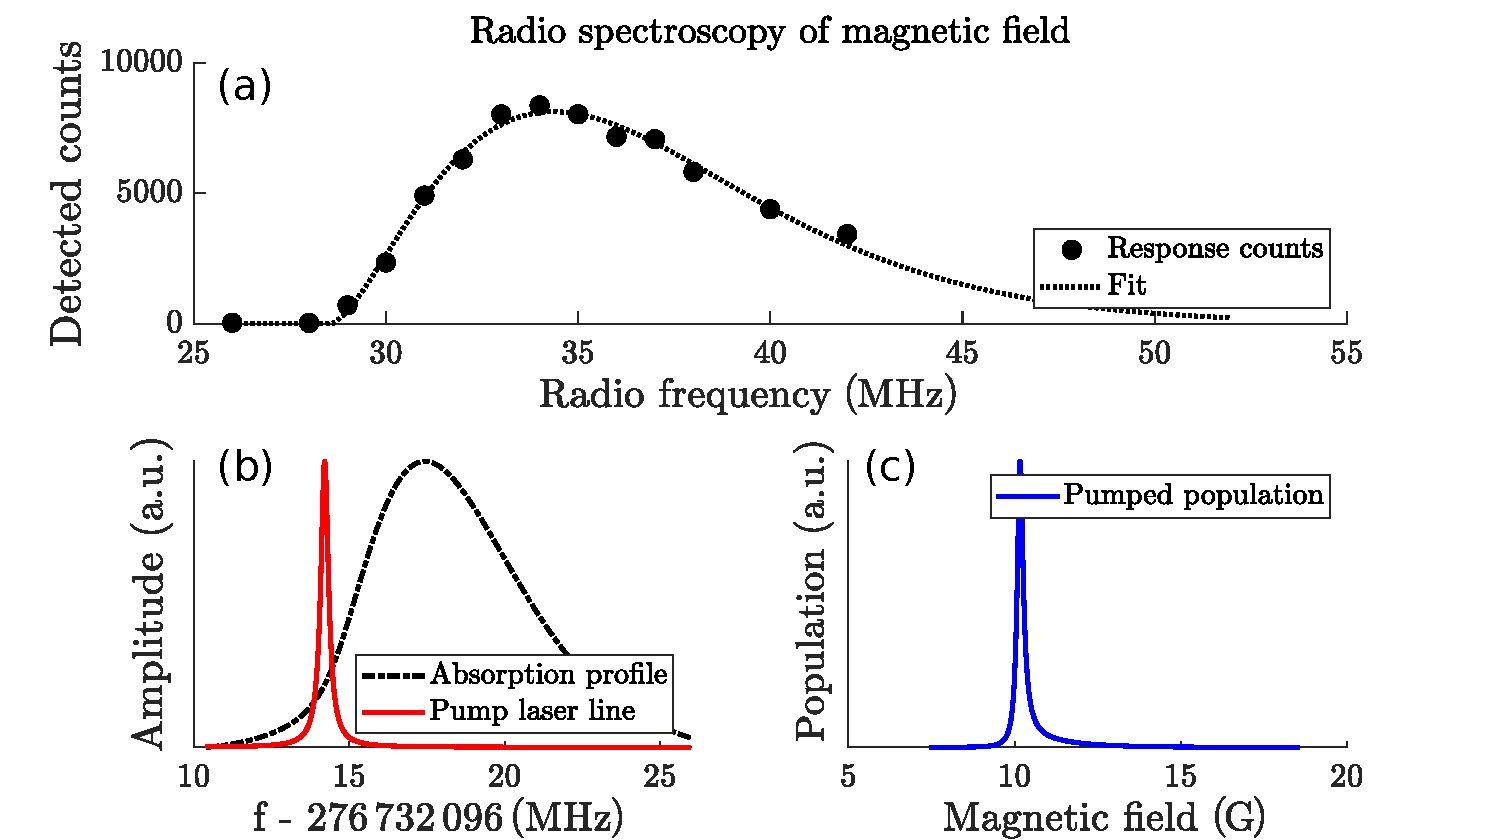
\includegraphics[width=0.5\textwidth]{fig/spectroscopy/rf_spec_subfig-eps-converted-to.pdf}
% \caption{Determination of magnetic field for Zeeman shift correction.
% 	The number $n_\text{D}$ of atoms detected after probing the trap with 300ms of RF radiation is shown in (a) versus the frequency of the applied radiation.
% 	Each point is an average of three shots.
% 	A Bose-Einstein fit models the population density $n_\text{T}$ of the $2\triplet S_1$ state at a given field strength.
% 	In (b) the calculated absorption profile of the gas in the vicinity of the 1083nm pump transition is shown, along with the spectral profile of the pump laser.
% 	The pump laser selectively excites atoms with a certain Zeeman splitting, leading to a population of atoms in the $2\triplet P_2$ state (c) that is concentrated around a specific magnetic field strength.
% 	The resulting Zeeman broadening is dominated by the probe beam linewidth.}
% \label{fig:RF_spec}
% \end{figure}

% The probe laser can only excite atoms pumped into the $2\triplet P_2$ state, which has a population distributed over a finite range of magnetic field strengths.
	The peak of the response to the probe laser is given by the convolution of the probe laser spectrum and the density of pumped states over the magnetic field strengths.
	We identify the 

% Finite temp in non-uniform field would lead to Zeeman broadening as well as a shift...
	ungh run the trap sim?

Kinetic effects do not contribute any significant uncertainty in our frequency measurements, rather they just broaden the observed peaks.
	The pump light is applied by two counterpropagating beams, subtending angles of 15$^\circ$ and 195$^\circ$ relative to the direction of propagation of the probe beam.
	Photon absorption events contribute a recoil velocity of magnitude $\cos(15^\circ)\cdot\hbar k/m\approx6$mm/s, imparting a Doppler shift of order 1.4kHz.
	Atoms may absorb probe light after absorbing a photon from the pump beams, but not after decaying again, so the decay events do not contribute.
	Because there are two counterpropagating pump beams, the resulting contribution is a negligible broadening, especially in comparison with the thermal broadening.
	The difference between predicted and observed line widths is well accounted for by these broadening effects.


\begin{figure}
  \begin{minipage}[t]{0.6\textwidth}
  \vspace{0pt}
  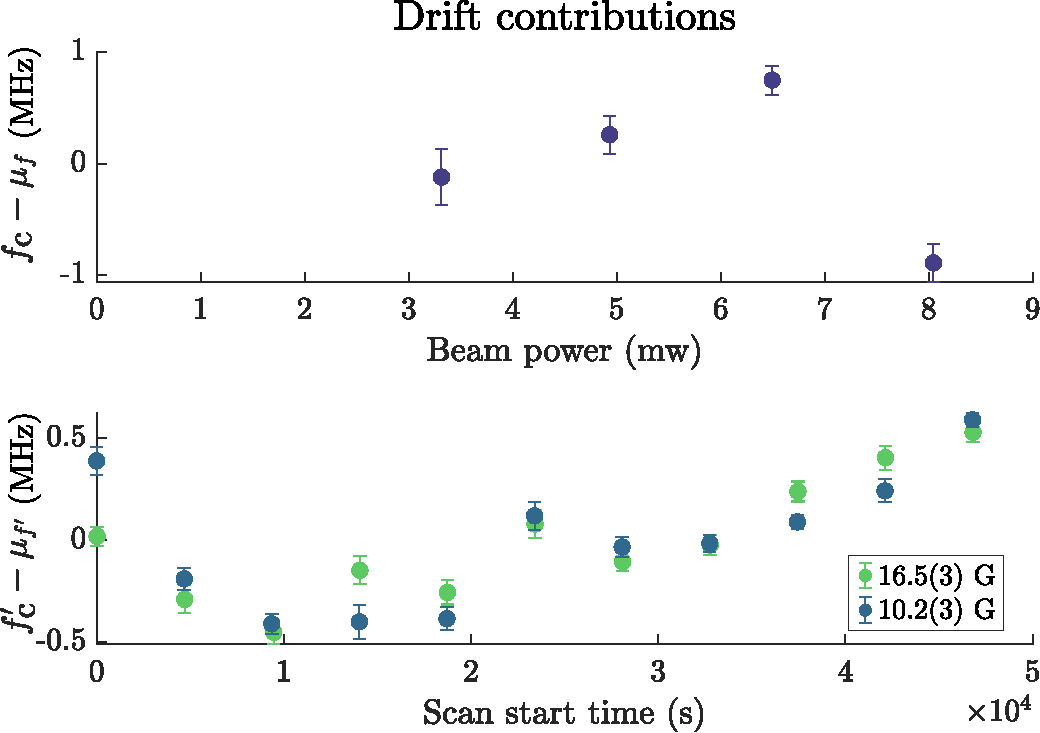
\includegraphics[width=\textwidth]{fig/spectroscopy/power-drift-combined-eps-converted-to.pdf}
  \end{minipage}\hfill
  \begin{minipage}[t]{0.38\textwidth}
  \vspace{0pt}
\caption{Top: Variation in fitted centre frequency for single scans across the $5\triplet D_1$ line versus applied laser power.
	The measurements at increasing beam power were not taken in chronological order Bottom: Variation in fit center frequency for the $2\triplet P_2 - 5\singlet D_2$ between scans.
	The value of the fitted peak centre $f_\textrm{c}$ is shown for each field strength, relative to the mean $\mu$ of all values for that field strength.}
\label{fig:power_drift_combined}
  \end{minipage}
\end{figure}

% \begin{figure}
% 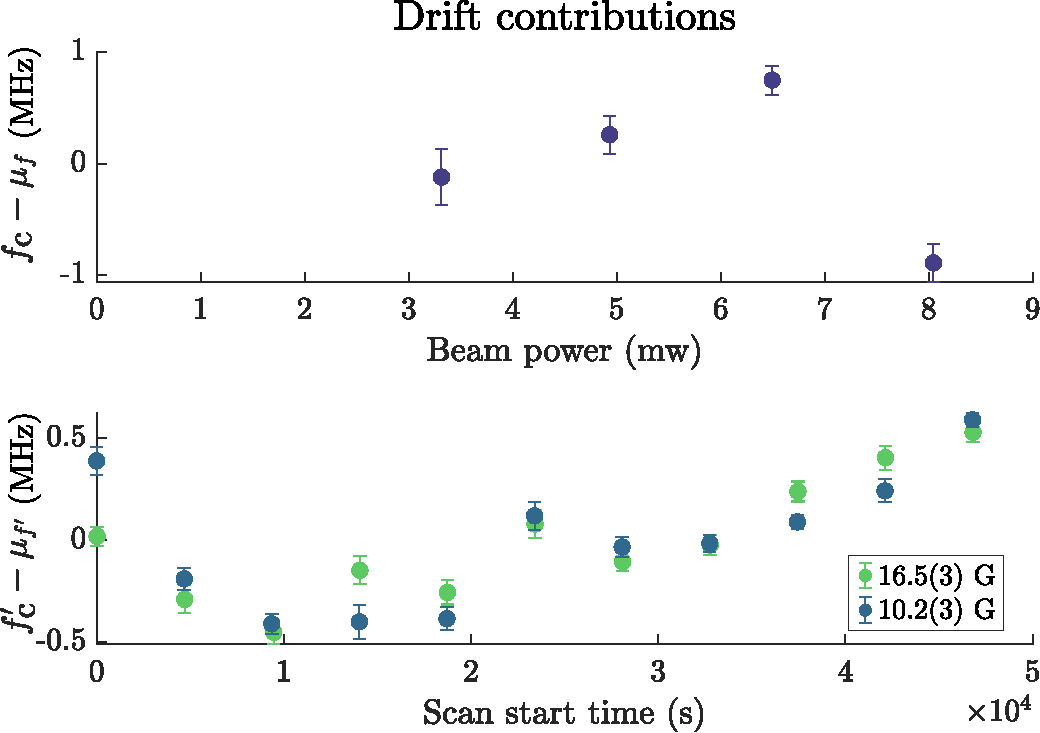
\includegraphics[width=0.48\textwidth]{fig/spectroscopy/power-drift-combined-eps-converted-to.pdf}
% \caption{Top: Variation in fitted centre frequency for single scans across the $5\triplet D_1$ line versus applied laser power.
% 	The measurements at increasing beam power were not taken in chronological order Bottom: Variation in fit center frequency for the $2\triplet P_2 - 5\singlet D_2$ between scans.
% 	The value of the fitted peak centre $f_\textrm{c}$ is shown for each field strength, relative to the mean $\mu$ of all values for that field strength.}
% \label{fig:power_drift_combined}
% \end{figure}

Other precision measurements of transition frequencies have been shown to be subject to line pulling effects \cite{Marsman15,Marsman15PRA}.
	These effects arise in multilevel transitions because of interference between the laser-driven transition path and off-resonant driving through transitions with neighbouring intermediate states.
	We estimate the worst-case shift by $w_{\text{pump}}^2/\Delta_{2P} + w_{\text{probe}}^2/\Delta_{5L}$ \cite{Marsman15,Marsman15PRA}, where the $w$ terms are the linewidths of the pump and probe transitions, and the $\Delta$ terms are the Zeeman splittings between the sublevels of the pump and target states.
	The largest estimate among all the reported transitions is 500kHz.
	While this uncertainty is dominated by other effects in our experiment, it will be important to understand them for improved measurements in the future.


We determine no significant contribution from the AC Stark effect.
	During measurements of the $5\triplet D_1$ transition with varying probe beam powers, we found that any dependence of the centre frequency on the laser power was dominated by the drift in the wavemeter output, as shown in Fig.
	\ref{fig:power_drift_combined}.
	For the triplet-singlet transition, the increase in laser intensity is more than compensated for by the reduced dipole matrix element, and hence we come to the same conclusion.
	



\section{Discussion}

We performed multilevel laser absorption spectroscopy of excited state transitions in ultracold helium.
	This includes the first observation (to our knowledge) of the forbidden $2\triplet P_2 - 5\singlet D_2$ transition.
	Our measurements agree with current predictions within our error budget and suggest that the $93\sigma$ difference between previous measurements \cite{Martin60} and predictions \cite{Morton06} of the $\PStateManifold_2  -  \UpperS$ and $\PStateManifold_2  -  \UpperStateManifold$ intervals are due to an unkown systematic error \footnote{As a historical note on the advancement of experimental methods, Martin's measurements were made using a nitrogen-cooled helium discharge lamp fed through an in-vacuum prism onto photographic plates, on which the line separations were measured by hand with a ruler.}.
	%Our work provides five contributions to the NIST database of atomic spectral lines.
	

The techniques described here are readily extensible to other opportunities in $^4$He structure measurements.
	For example, while there is an outstanding 7.4$\sigma$ disagreement between the predicted and observed singlet-triplet interval for the n=3 level in $^3$He \cite{Morton06,Derouard80}, the corresponding transition in $^4$He has never been directly measured.
	An indirect measurement in $^4$He could be made with the techniques described here by taking the difference betweeen the $2\triplet P_2 - 3\triplet D_2$ and $2\triplet P_2 - 3\singlet D_2$ transitions near 587.6nm and 587.4nm.
	While the latter transition is also spin-forbidden, it is predicted to be an order of magnitude stronger than the $2\triplet P_2 - 5\singlet D_2$ transition reported here \cite{Morton06}.

{Further, energies of other $2L-nD$ transitions in $^4$He are a few MHz larger than predicted, apparently independent of $L$ \cite{Wienczek19,Yerokhin20}.
	Our results deviate from this trend, and invite independent verification.
	Further study of transitions between states from different shells to MHz precision or better, in particular the prospective study of the $2\triplet P - 3 D$ intervals, would also provide further clarification.}

Simply exchanging the light source would suffice to make these measurements, but a definitive comparison with theory would require an improved frequency reference.
	For instance, the hypothetical $10/n^3$ MHz shift could be checked by a measurement of the $2~P-n~D$ transitions accurate to sub-MHz precision.
	The associated theoretical uncertainties are about this size, dominated by the 700 kHz uncertainty in the lower state \cite{Pachucki17,Wienczek19}.
	As the $\alpha^7$ terms could improve the theoretical accuracy to as little as 10kHz \cite{Pachucki17}, this more challenging precision appears to be a more appropriate budget, and readily achievable with current methods.
	Reference-locked optical frequency combs can readily achieve kHz accuracy or better \cite{Luo15,Rengelink18}.
	Magnetic field strengths can be determined by RF spectroscopy with sub-kHz accuracy and so would not present a serious limitation.
	Improving the AOM frequency stability would provide sufficient accuracy to account for laser-induced stark shifts, likely leaving systematic drifts as the dominant source of error.

Extending these methods to direct measurements on $^3$He would also permit isotope shift measurements from forbidden excited-state transitions in $\triplet$He.
	Theoretical calculations of isotope shifts are already accurate to the sub-kHz level, so such measurements would be even more demanding than the prospects above.
	Existing demonstrations of comparable accuracy \cite{Rengelink18} show such measurements are worthy challenges whose completion can access femtoscale nuclear structure information via optical atomic spectroscopy.


\vfill

\begin{flushright}
\emph{
``Immediately you would like to know where this number for a coupling comes from:\\ 
is it related to pi or perhaps to the base of natural logarithms? Nobody knows.\\
It's one of the greatest damn mysteries of physics: a magic number that\\
comes to us with no understanding by man.
	You might say the \\
``hand of God" wrote that number, and ``we don't know how\\
He pushed his pencil." We know what kind of a dance to\\
 do experimentally to measure this number very accurately,\\
  but we don't know what kind of dance to do on the computer\\
to make this number come out, without putting it in secretly!"}\\
- Richard P.
	Feynman \footnote{\emph{QED: The Strange Theory of Light and Matter}.
	Princeton University Press.
	p.
	129.
	(1985)}
\end{flushright}



% * Dipole operator -> Clebsch-Gordan again
% % Fermi's golden rule: $\Gamma_{ij} = \braket{i, H_{dip}, j}/\hbar$ ?

% This comes from the atom in an oscillating electric field.
	% The Hamiltonian is
% % $$
% % \hat{H} = \hat{H}_{\alpha} + \hat{H}_{\omega} + H_{int}\\
% 		% & H_{nLm_lSm_s} + \frac{\hat{n_\gamma}+1}/{2}\hbar\omega_\gamma ...\\
% 				% + \int H(\alpha,\omega) d\omega
% % $$
% where $\alpha$ and $\omega$ denote the Hilbert spaces of the atom and of the bosonic field, respectively, and $H_{\int}$ is the interaction term.
	% In the plane wave picture, we can think of the electromagnetic field, with modes $\omega$, then a \emph{coherent} field has several connotations and implications.
	 

% Classically, we can also describe the electromagnetic field as a vector field $E\times X$ with $E(x): (x,y,z,t) \rightarrow \mathcal{S(x)}$, where $S(x)$ is the Stokes vector at each point.

% \end{itemize}

% 	This chapter describes two measurement campaigns of electronic transition energies in Helium.
	% First, I recount the method and used to measure the energy splittings between the $\PStateManifold_2$ state and a collection of states in the $n=5$ manifold, including the first observation of a transition between the $2\triplet P$ and $5\singlet D$ manifolds in Helium.
	% Second, I describe two methods used to measure the energy and the transition lifetime of the forbidden $2\triplet S_2\rightarrow 3\triplet S_1$ transition, the weakest electronic transition observed in a neutral atom to date, previously considered too weak to be measured\cite{Lach01}.
	

% 	The work described in this chapter provided the basis for the following publications:

% 	\begin{itemize}
% 		\item K.F.Thomas, J.A.Ross, B.M.Henson, D.K.Shin, K.G.H.Baldwin, S.S.Hodgman, and A.G.Truscott, Direct Measurement of the Forbidden $2\triplet S_1\rightarrow 3\triplet S_1$ Atomic Transition in Helium, \emph{Journal} \textbf{issue}(2020), \href{<https://arxiv.org/abs/2002.04811>}{<arXiv>}
% 		\item J.A.Ross,  K.F.Thomas,  B.M.Henson,  D.Cocks, S.S.Hodgman,  K.G.H.Baldwin,  and  A.G.Truscott, Measurement of spin-forbidden excited-state transitions in metastable helium, \emph{Journal}, \textbf{issue} (2020) 
% 	\end{itemize}
% 	% Spec paper
% 	% forbidden paper

% 	\newpage

% \section{Measurement of five $2\triplet  P_2\rightarrow 5L$ transition energies}\label{sec:he-trans}

% 	Some of the $\PStateManifold_2\rightarrow5_D$ transitions were observed by Martin in 1960\cite{Martin60}, but his measurements are in stark disagreement with present predictions\cite{Wiese09} by about 13 GHz.
	% Further, in the NIST database, the transition energies to the $5\triplet D$ states are all identical\.
	% Indeed, in Martin's original paper, he only quotes measurements from $\PStateManifold$ to the $5D$ level in general, indicating that his equipment did not have the resolving power to distinguish the fine structure of the $5\triplet D$ state.
	% Martin was also unable to distinguish transitions to the $5\singlet D$ level, probably due to its proximity to the $5\triplet D$ lines .
	% The contents of this chapter are complementary to the following publications:

% \subsection{Tests of fundamental physics with helium spectroscopy}

% 	Quantum electrodynamics (QED) describes the interaction of light and matter.
	% It is the most accurate quantitative physical theory to date.
	% The state of the art of experimental atomic spectroscopy is sufficient to match theoretical uncertainties in table-scale experiments, signalling an era in which atomic physics laboratories can contribute to tests of fundamental physics.
	% Atomic structure predictions are made using the theory of QED and assuming the CODATA values of the fundamental constants.
	% With the present accuracy of theory and experiment, it is possible to back-calculate from observed data and constrain fundamental constants.
	% Schwartz identified opportunity to determine the fine structure constant in Helium in 1964, noting that the $\PStateManifold$ fine structure intervals are subject to strong QED effects, but have lifetimes about an order of magnitude larger than the same states in Hydrogen.
	

% 	The ongoing theoretical campaign \cite{Pachucki15,Pachucki17,Pachucki11,Pachucki10,Morton12,Morton06,Patkos16,Patkos17} has reached sufficient accuracy to obtain a $4\sigma$ discrepancy for the squared charge radii difference between Helium-3 and Helium-4 obtained from the $\MetastableState \rightarrow \PStateManifold$ and the $\MetastableState\rightarrow {2\singlet S_{0}}$ transitions\cite{Pachucki15}.
	

% 	A comprehensive tabulation of Helium levels and transition rates was compiled by Wiese and Fuhr in 2009 \cite{Wiese09}, based on the extensive work by Pachucki, Yerokhin, Morton, Drake, and collaborators.
	% These calculations were recently verified by Zhang et al \cite{Zhang15}.
	% Predictions are made using the theory of QED and assuming the CODATA values of the fundamental constants.
	% With the present accuracy of theory and experiment, it is possible to back-calculate from observed data and constrain fundamental constants.

% 	The theoretical campaign \cite{Pachucki15,Pachucki17,Pachucki11,Pachucki10,Morton12,Morton06,Patkos16,Patkos17}, has reached order $\alpha^6m^2/M$ in both singlet and triplet states states\cite{Patkos16,Patkos17}.
	% Efforts are ongoing to compute the $\alpha^7$ contributions expected to allow determination of the Helium nuclear charge radius accurate to 1\%\cite{Pachucki17}.
	% Already, there is sufficient accuracy to obtain a $4\sigma$ discrepancy between squared charge radii difference between Helium-3 and Helium-4 obtained from the $\MetastableState \rightarrow \PStateManifold$ and the the $\MetastableState\rightarrow {2\singlet S_{0}}$ transitions in each, namely $\delta r^2 = 1.069(3)~\textrm{fm}^2$ and $\delta r^2 = 1.061(3)~\textrm{fm}^2$ for the former and $\delta r^2 = 1.027(11)~\textrm{fm}^2$ for the latter\cite{Pachucki15}.
	% With improved calculations of $\PStateManifold$ splitting to 1.7kHz\cite{Pachucki17}, experimental precision is now the limiting factor in determining the isotope shift.
	

% 	Cancio Pastor \textit{et al.} used Helium spectroscopy to make the then-most accurate Lamb shift measurement in any atomic system\cite{Pastor04}.
	% Six years later, Smiciklas \textit{et al.} measured the $\PStateManifold$ fine structure splitting to sub-kilohertz precision, determining fine structure constant to 5ppb\cite{Smiciklas10}.
	% Measurement of the $2^3P-2^3S$ spacing to within 1.4kHz would determine the nuclear charge radius to below 0.1\%, better than expected from the muonic helium Lamb shift\cite{Wienczek19}.
	 

% 	Recently Kato \emph{et al} refined measurements of the $2\triplet  P_2\rightarrow2\triplet  P_1$ to 25Hz accuracy, which can constrain $\alpha$ to less than one ppb in conjunction with similarly accurate measurement of the $2\triplet  P_1\rightarrow2\triplet  P_0$ transition and QED corrections of order $\alpha^7$ \cite{Kato18}.
	% Ongoing efforts \cite{Pachucki17} to obtain these corrections will also allow determination of absolute nuclear charge radii accurate to better than 1\%, complementary to ongoing investigation of the proton radius puzzle.

% 	Curiously, measured transition energies from the $n=2$ manifold to the 3D levels are about 1MHz larger than predicted.
	% Assuming the usual $1/n^3$ scaling of QED effects, such an anomaly would imply a deviation of $10/n^3$ MHz in ionization energy for an arbitrary state, motivating further study of transitions between states from different shells \cite{Wienczek19}.
	% In this work, we measure five transitions from the $2^3P_2$ state to the $n=5$ level, improving on the precision of past measurements\cite{Martin60} by order of magnitude.
	% We resolve lines from the $\PStateManifold_2$ to the $\UpperSingletStates$ states individually for the first time.
	% We make the first observation of the spin-forbidden $2^3P_2\rightarrow5^1D_2$ transition in Helium.
	% Future measurements with greater precision could assist efforts to resolve a 7.5$\sigma$ disagreement between the predicted and observed $n=3$ singlet-triplet splitting\cite{Morton06}.

% 	\begin{figure}[b]
% 	    \centering
% 	    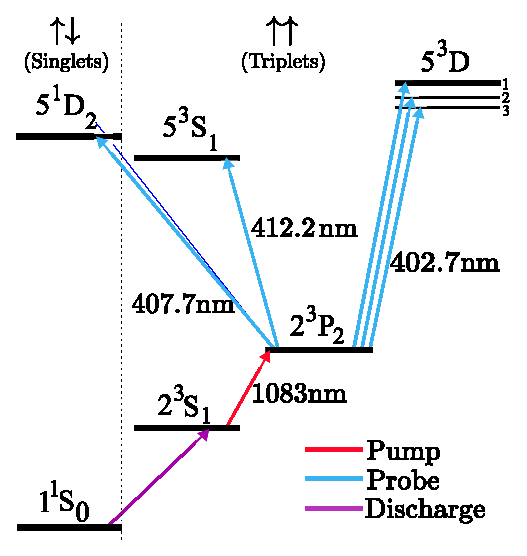
\includegraphics[width=\textwidth]{fig/Spectroscopy/level_diagram_tight_latex.eps}
% 	    \caption{A level diagram for the helium atom.
	% The transitions measured in this work (blue), are driven by a tunable laser referred to in text as the 'probe'.
	% The cooling transition (red) is referred to as 'pump' throughout the paper and populates the lower state of the target transitions.
	 % The doubly forbidden $1\singlet S_0\rightarrow2\triplet  S_1$ transition is excited in a high voltage discharge cell.
	% Transitions between the singlet and triplet manifolds (left and right of dotted line) are forbidden in the dipole approximation.
	% The level splittings are not to scale.}
% 	    \label{fig:lvl_diag}
% 	\end{figure}

% \subsection{Detection scheme}\label{ssec:spec-detection}
% \begin{itemize}
% 	\item Setup - alignment
% 	\item Procedure
% 	\item Mechanism
% 	\item Calibrations
% 	\item Analysis
% \end{itemize}

% \subsubsection{Procedure}
% 	We use a micrometer translation mount on the final lens to align the beam on the Helium sample.
	% We locate the transitions approximately by using the maximum available laser power at the predicted frequency, and then reducing the power and adjusting the frequency set point until the signal no longer saturates at the peak.
	% We then scan the set point of the laser across the transition to obtain the transition signal.
% 	The beam was initially aligned by tuning the probe beam to the predicted value of the 53S1 transition and operating with the maximum available power.
	% Although the uncertainy in wavemeter accuracy was larger than the transition linewidth, by operating well above the saturation intensity, the transition was broaded by tens of MHz and so the WM error was less significant.
	% When scanning the beam pointing across the expected target region, approximate alignment was signaled by a dramatic loss of atom number.
	% When the signal saturated, the power was lowered until the signal was just above the noise floor, and then scanning resumed.
	% This process iterated a few times until the maximum attainable signal was below saturation - that is, when for fixed power one could not completely destroy the trap.
	% Notice there are three kinds of saturation here: Atomic population saturation, detector saturation, and signal saturation when you run out of atoms.
	% perhaps the term `dynamic range' would be more suited to the latter\ldots{} Something to think about.

% 	During the calibration shots, we also block the beam with a mirror mounted on an automatic translation mount.
	% The profile and polarization of the beam are determined with lenses and waveplates prior to vacuum entry.
	% The measurement sequence consists of measurement shots with each of the two magnetic field strengths followed by calibration shots, wherein the laser beam is blocked and switched off.
	% We calibrate the wavemeter before each transition measurement.
	% Analysis of the wavemeter stability suggests that calibration drift is not a significant source of error, as discussed in the supplementary materials.

% 	The method therefore consists of alternating measurement trials with control trials, wherein the laser beam is blocked before the fibre coupler with a flipper mirror.
	% At the moment I use an interpolation, but I might want to try using a model-based estimate of the atom number.
	% Either way, there is going to be some error in the number estimation.
	% It's probably small.
	% The difference between the interpolated, unperturbed atom number and the detected number in the measurement trials is affected by the quantum efficiency and the introduced uncertainty in atom number.

% 	The polarization of the light was fixed with the waveplates before the chamber.
	% Can you tell handedness just by relative angle of waveplates? We hypothesized that the initial state of the atoms during the cooling phase was in the m=2 state, as the optics are configured to drive with a sigma+ beam during the in-trap cooling stage.
	% I verified this by driving with plane-polarized light (in the atom frame - put some trap sim in to show where the field points), which is a linear combination of sigma+ and sigma- light.
	% If there were atoms in initial states other than the m=2, then when driving to the 53S1 state, one would observe multiple peaks.
	% Instead, only one peak was observed, which vanished when the probe beam was set to sigma+ light.
	% (I think check the data).

% 	The measurements are taken at two different background field strengths.
	% Therefore the detuning from cooling resonance is X and Y MHz in each stage, respectively.
	% These values were calibrated independently by an RF spectroscopy technique.
	% This allows empirical extrapolation to the field-free transition energy by correcting for the calculated Zeeman shift of the centre frequency of each measured line.


% % Peak intensity is ~ total power x 1e3 /m^2 for large beam
% \begin{table}
% \begin{tabular}{|c|c|c|c|c|}
% \hline
% Line & Beam waist (cm) & Beam power (mW) &  Peak intensity (W/m$^2$) & Exposure time (ms)\\
% \hline
% $5\triplet S_1$  & 4.1 &  2.73(1) & 3.1(2) & 100 \\
% $5\triplet D_1$  & 4.1 &  4.5(1) & 5.2(1) & 150\\
% $5\triplet D_2,3$& 4.1 &  8.6(1) & 9.9(1) & 250  \\
% $5\singlet D_2$  & 0.1 &  10(2) & 6.3E3 & 100 \\
% \end{tabular}
% \label{tab:spec-beamparams}
% \caption{Probe beam parameters}
% \end{table}
% \begin{table}
% \begin{tabular}{|c|c|c|c|c|}
% \hline
% Stage & Beam power & AOM detuning & Peak intensity & Transition detuning\\
% \hline
% \end{tabular}
% \label{tab:spec-pumpparams}
% \caption{Pump beam parameters}
% \end{table}

% \subsubsection{Data acquisition}
% 	\com{This probably goes in the Intro/BEC machine part}

% 	Following the laser interrogation, the remaining atoms are gradually outcoupled from the trap with a pulsed atom laser.
	% At the beginning of each shot, the LabView control interface writes a line to the log file with the parameters \verb|timestamp, laser_setpt, shot_type| where \verb|shot_type| is either \verb|stage_1|, \verb|stage_2|, or \verb|calibration|.
	% When importing the data into the processing scripts, the 

% 	 As the laser set point is fixed for sets of three shots (one per field setting), 


% \subsubsection{Mechanism of action}
% 	
% 	To drive the transitions from the 23P2 state to the states in the n=5 manifold, I use the probe beam to disturb the near-resonant optical molasses cooling stage of the experiment.
	% This follows the MOT loading and precedes evaporative cooling, and operates with XYZ beam parameters for XXX ms, and then with ABC beam parameters for YYY ms.
	% I calculate that during these stages, the excited-state population is ZZZ per cent, which are then susceptible to scattering photons from the probe beam.

% 	I used the evaporative cooling sequence as a transducer between scattering-induced heating of the cloud and the final condensed number.
	% I will present a quantitative sketch of the mechanism below, but one can also take a heuristic understanding from the following argument:

% 	The evaporative cooling we use to achieve Bose-Einstein condensation has stringent tolerances on initial phase space density, which increases with number and at lower temperatures.
	% Tuning a radio chirp to the spin-flip transition from a trapped to an untrapped state and sweeping down to lower energies, higher-energy atoms are removed, the cloud rethermalizes at a lower temperature, and the phase space density increases.
	% Higher-energy atoms spend time further from the centre of a harmonic magnetic trap.
	% So, scattering photons from the probe beam heat the cloud, leading widening the velocity distribution, which drives more of the atoms into resonance with the radio chirp.
	% The final temperature is determined by the endpoint of the radio chirp.
	% Resonance with the probe light manifests as a signal in a reduction of the final population of the condensate.

% 	As I said, an essential part of our BEC production is an optical cooling and spin-polarizing stage which precedes the loading of our magnetic trap.
	% This ensures a nice large atom number and low temperature.
	% This give us a nice big phase space density, a dimensionless number which compares the length scale of quantum interference, the de Broglie wavelength, with the interparticle spacing given by the particle density n.~So, disturbances to this initial condition by atom loss or heating will reduce the phase space density input to the evaporation stage.
	% The Bose-Einstein condensation threshold occurs when the phase space density crosses about 2 - for comparison, atmosphere has a phase space density about one ten millionth of that.
	% One can therefore think of the RF evaporation as a phase space amplifier in the following way:

% 	Evaporative cooling works by creating a resonance between trapped and untrapped magnetic states of atoms with a specific Zeeman splitting by exposing the cloud to radio frequency radiation.
	% Energetic atoms travel up the magnetic field gradient, shown by the thickness of the purple lines, to the ellipsoidal shell defined by a fixed field strength at which the atoms resonate with the radio waves.
	% The atoms are then transferred into free states and leave the trap, taking with an amount of energy greater than the ensemble average.
	% This basically cuts out the upper tail of the Maxwell-Boltzmann distribution, driving down the atom number, but also the temperature once the cloud rethermalizes.
	% If you get this right, you continuously increase the phase space density by making the cloud cooler and smaller, until you get to BEC.
	% The endpoint of the RF chirp fixes an upper bound to the energy of the trapped atoms, and hence a temperature.
	% Then the phase space density can be estimated by counting the number of atoms you have left.
	% We measure this atom number using Helium's unique detectability - by applying broadband radio pulses to the trap we free about 0.5\% of the atoms at a time, creating a series of pulses of coherent matter waves, known as an atom laser.
	% This resolves on our detector as a series of discrete particle detection events, which we sum up with an abacus.
	% So by controlling our independent variable, the applied laser frequency, we have a gain mechanism that allows us to measure the dependent variable, which is the phase space density reduction by resonant scattering of photons from the probe beam.

% \subsubsection{Calibration measurements}

% 	After the probe is applied during the optical molasses cooling, we use a standard forced evaporative cooling procedure.
	% At the end of the sequence the atoms are in the metastable $2^3S_1$ state which exhibits a 19.8eV ground state separation.
	% This internal energy enables single-atom detection by a multi-channel plate and delay-line detector stack with an efficiency of 8 per cent\cite{Manning10} to determine the atom number loss.
	% We use a pulsed atom laser \cite{Manning10,Henson18} to transfer atoms to the untrapped state and avoid detector saturation.


% 	A translation mount on the final lens gives us micrometer precision in the placement of the focal point on the beam, which we use to align the beam on the trap, threading a ten micron needle in the dark 20 micro-radian accuracy.


% 	\begin{table}
% 	\label{tab:aom_calibration}
% 	\begin{tabular}{|c|c|c|c|}
% 		\hline
% 		RF centre frequency & Calibrated field strength (G) & AOM frequency (MHz) & Detuning (MHz) \\
% 		\hline
% 		XXX & 18 & 138 & 0.5\\
% 		XXX & 11 & 133.6 & 2\\
% 		\hline
% 	\end{tabular}
% 	\end{table}
% 	AO offsets 138MHz and 133.6MHz ?
% 	cooling transition is split 25.55 MHz, and 16.002 in stage 2
% 	Therefore the beams are (ish) detuned 0.5 and 2MHz respectively

% \subsubsection{Analysis}
% 	In this section I describe the data processing method used for the peaks, using the $5\singlet D_2$ line as an example.

% \subsection{Findings}\label{ssec:spec-findings}

% \subsubsection{Results}

% 	\begin{figure*}
% 	  % \includegraphics[width=\textwidth]{fig/Spectroscopy/pub_lines_j1.eps}
% 	  \caption{Measured line profiles for the $\PStateManifold_2\rightarrow 5\triplet  S_1$ (left) and   $\PStateManifold_2\rightarrow 5\triplet  D_1$ (right) transitions, with Lorentzian fits.
	% On the horizontal axis is the probe laser frequency $\nu$, relative to the theoretical prediction for the magnetic field-free splitting.
	% The vertical axis is the response as measured by atom number loss relative to the calibration shots.
	% Theoretical predictions (vertical bars) are Zeeman shifted from the zero-field value according to the field calibration, with uncertainty (horizontal bars) dominated by uncertainty in background field strength.
	% Lines obtained by measuring against an 18G and 11G background field are shown in red and blue, respectively.
	% }
% 	  \label{fig:simple_lines}
% 	\end{figure*}


% \subsection{Determination of transition energies}\label{ssec:spec-processing}


% \begin{figure}
% 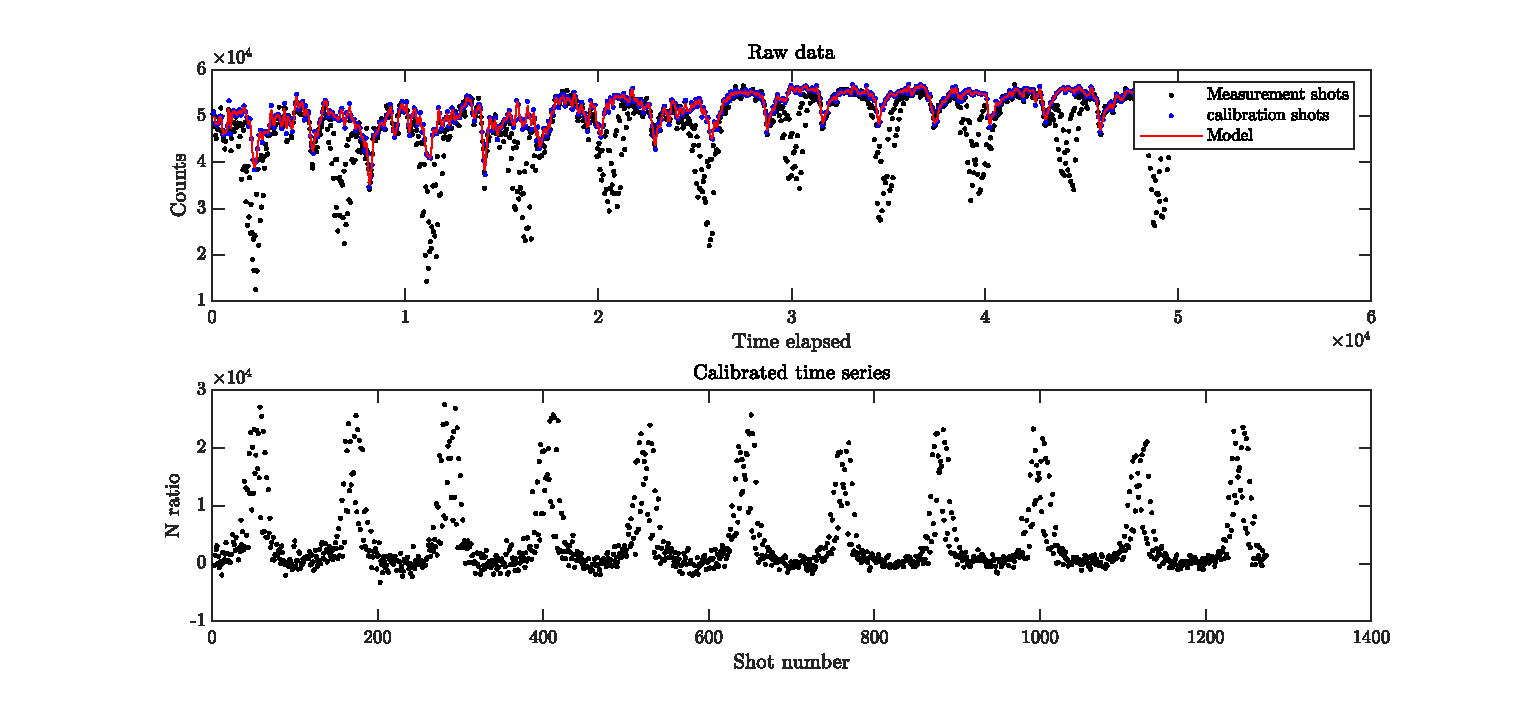
\includegraphics[width=\textwidth]{fig/spectroscopy/calib_model_51D2.eps}
% \label{}
% \caption{}
% \end{figure}

% \begin{figure}
% 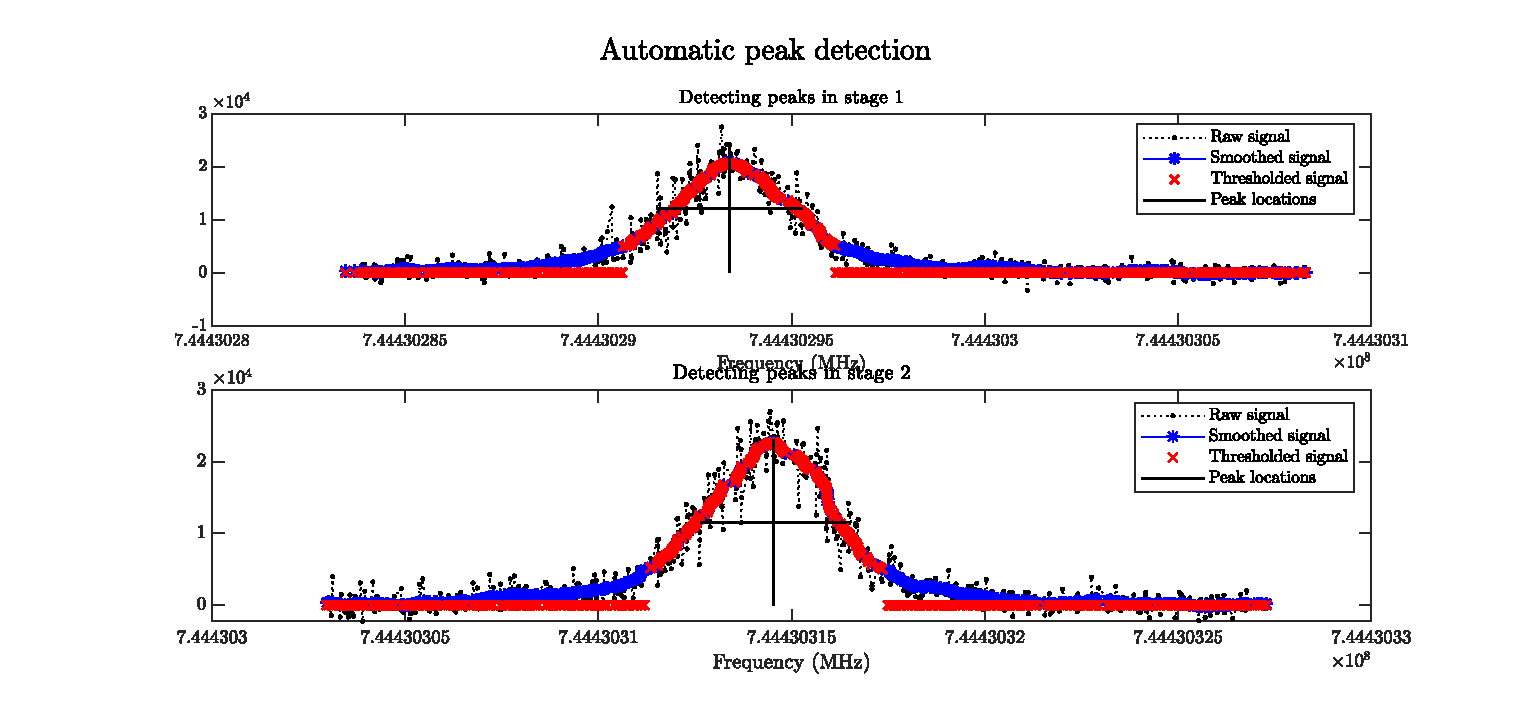
\includegraphics[width=\textwidth]{fig/spectroscopy/auto_peak_detect_51D2.eps}
% \label{}
% \caption{}
% \end{figure}

% \begin{figure}
% 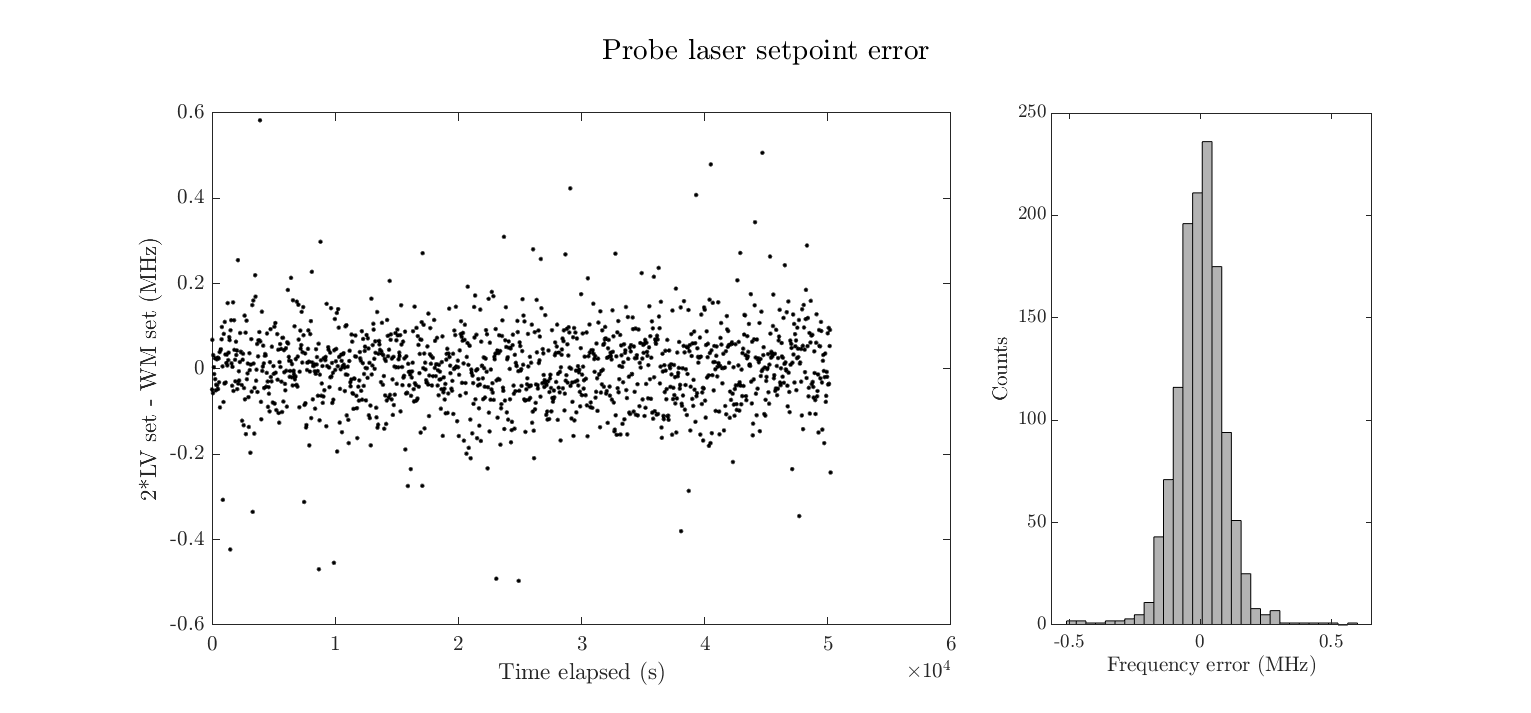
\includegraphics[width=\textwidth]{fig/spectroscopy/probe_set_err_51D2.eps}
% \label{}
% \caption{}
% \end{figure}

% \begin{figure}
% 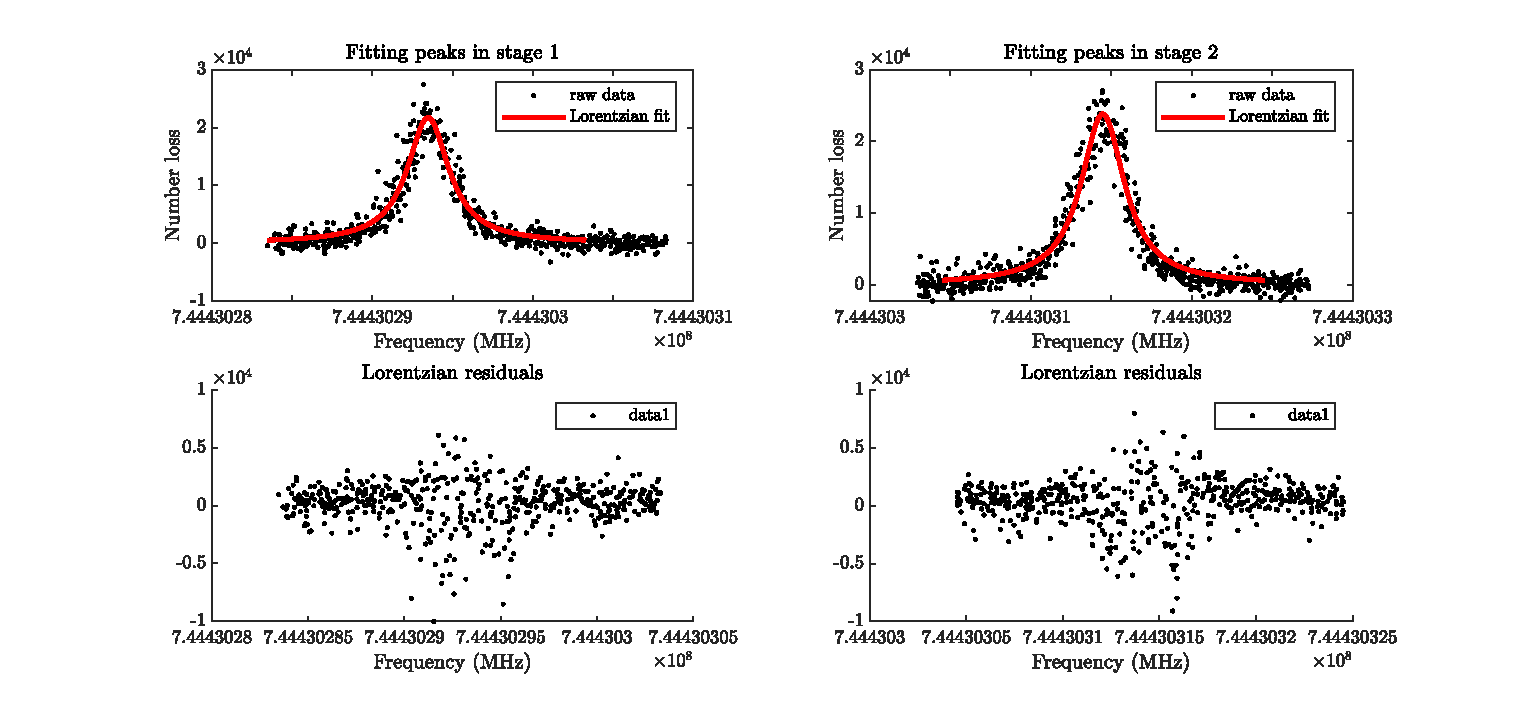
\includegraphics[width=\textwidth]{fig/spectroscopy/fitting_peaks_51D2.eps}
% \label{}
% \caption{}
% \end{figure}

% 	We empirically extrapolate to the field-free transition energy by correcting for the Zeeman shift in the observed lines.
	% The exposure time and intensity varied among measurements to avoid saturation.
	

% 	The table below displays the results of the measurements, including predicted linewidths.
	% In the case of the 23S1-33S1, the measured Einstein A coefficient is also listed.
	% These measurements are accurate to a few hundred parts per billion, and their accuracy is limited by the absolute accuracy of the wavemeter we used as a reference for the laser lock.
	% Within the accuracy stated by the manufacturer, these results are consistent with the predictions of QED.
	% Of the six lines measured, three have been resolved individually for the first time, and two have not been recorded elsewhere.
	% The centre frequencies are obtained by fitting Lorentzian profiles to the atom loss spectra.
	% Have a look at residuals; what are the expected broadening effects? What are the expected systematic errors? Error budget goes here also.
		

% 	Ah.
	% The CG madness is only needed for the triplet D states.
	% The singlet D and the triplet S have zero total angular momentum for the spin and orbital dof, respectively, so the basis is trivial and in these cases, we can use the linear extrapolation method with no worries.
	% What about the 2 3P2? Oh - I missed a point, which is the presence of other nearby levels.
	% For the singlet D, that's done, it's unique, as S=0.
	% And for the triplet S, also, as L=0.
	%  Not so for the 2 3P2.
	% But they're several GHz away so that shouldn't be a problem at all.
	% Well, then that's cleared up! Great.
	% Now to write this nonsense up.
	% Start concise in the paper, then we can expand it here.
	% later.

% % A and Sum A from \cite{Drake07}
% % Triplet D: 8.3444E+02 1.3929E+07
% % 5 3S1 line 2.4738E+06 sum 9.2072E+06
% % 5 3DJ sum 1.6412E+07
% % 	Lines
% % 	J=1 3.2224E+05
% % 	J=2 2.8999E+06
% % 	J=3 1.1601E+07
% % 5 1D FROM 2 3P1 402.7151538 nm
% % the 2 3P J=1-2 interval is 2291.177 MHz from Zheng
% % line 8.3444E+02 sum 1.3929E+07
			
% % Two-peak results STAGE 1:

% % Widths: [4.30,5.73,3.03,3.14]
% % Two-peak results STAGE 2:
% % Centres: [744396208.29,744396204.67,744396182.37,744396224.64]
% % Widths: [4.94,4.26,3.91,3.60]

% % Centres_1: [744396195.49,744396191.21,744396160.46,744396223.01]
% % Centres_2: [744396208.29,744396204.67,744396182.37,744396224.64]

% % 3S_1 727303244.61
% % 3D_3 744396209.66
% % 3D_2 744396228.89
% % 3D_1 744396512.43
% % 1D_2 744430344.53

% \begin{table*}
% 	\begin{tabular}{|c||c c|c|c|c|c|}
%     \hline
%         $|e\rangle$ & $f_\textrm{meas,1}$ & $f_\textrm{meas,2}$ & $f_{\textrm{field-free}}$   & $\Delta_\mathrm{theory}$ & $\textrm{FWHM}_\textrm{obs.}$ & $\textrm{FWHM}_\textrm{pred.}$  \\
%     \hline\hline
%         $5^3\mathrm{S}_1$    & 727,303,223.89 &				& 727,303,249(5)   &   4.4    &  3.12(40)& 9.21\\ % A = 
%                              & 727,303,234.04 &				&		& 			 & 		&	\\
%         \hline
%         $5^3\mathrm{D}_1$    & 744,396,453.41 &				& 744,396,496(21) & -16  &  5.79(62) & 16.4\\
%                              & 744,396,477.82 &				& 		& 			 & 	&	\\
%         \hline
%         $5^3\mathrm{D}_2$    &  744,396,191.21 & 744,396,223.01  & 744,396,217(22)  &  -12 & 4.18(50)  &16.4\\
%                              &  744,396,204.67 & 744,396,224.64 & 		& 			 &  &	\\
%         \hline
%         $5^3\mathrm{D}_3$    & 744,396,160.46 & 744,396,195.49 & 744,396,201(21) &  -8.7 & 4.04(12)   &16.4\\
%             			     & 744,396,182.37 & 744,396,208.29  & 		& 			 & 		&\\
%         \hline
%         $5^1\mathrm{D}_2$    & 744,430,295.37 &				& 744,430,347(21) &  2.5  & 3.21(13)  & 13.9\\
%                              & 744,430,316.37 &				& 		& 			 & 		& \\
%         \hline
% \end{tabular}
% \label{tab:spec-results}
% \caption{Summary of results (all in MHz) For each transition.
	% The measured frequencies are obtained in an ambient magnetic field of strength 18G (top row) and 11G (bottom row).
	% After correcting for the AOM and vapor cell shifts we extract the centre frequencies $f_{meas}$ from Lorentzian fits with statistical error at the $~ 10\textrm{kHz}$ level.
	% For the $5\triplet D_2$ and $5\triplet D_3$ states, each line shows the pair of transitions corresponding to the magnetic quantum number of the upper state $m_u=1$ and $m_u=2$, respectively.
	% After correcting for Zeeman shifts, the field-free energies $f_{\textrm{field-free}}$ are obtained, and shown with statistical error in parentheses.
	% We show the difference $\Delta_\mathrm{theory}$ between our measurements theoretical predictions \cite{Drake07}.
	% Observed line widths are the mean full width at half maximum $\textrm{FWHM}_\textrm{obs.}$ of a Lorentzian fit to each line, with theoretical predictions $\textrm{FWHM}_\textrm{pred.}$ from \cite{Drake07}.}
% \end{table*}
% 	\begin{figure}
% 	  % \includegraphics[width=\textwidth]{fig/Spectroscopy/pub_lines_5D1.eps}
% 	  \caption{Line profile for the spin-forbidden $\PStateManifold_2\rightarrow 5\singlet D_2$ transition, presented similarly to figure \ref{fig:simple_lines}.}
% 	  \label{fig:3D_1_line}
% 	\end{figure}


% 	\begin{figure}
% 	  % \includegraphics[width=\textwidth]{fig/Spectroscopy/pub_lines_5D2_3.eps}
% 	  \caption{Line profiles for the $\PStateManifold_2\rightarrow 5\triplet  D_{2}$ and $\PStateManifold_2\rightarrow 5\triplet  D_{3}$ transitions, driven by a mixure of $\sigma^-$ and $\pi$- polarized light and presented similarly to figure \ref{fig:simple_lines} and \ref{fig:3D_1_line}.
	% The large central peak is the overlap of two peaks, the transitions to the XXX and YYY lines, which are nearly degenerate for the entire operational range of our background magnetic field.}
% 	  \label{fig:3D_23_lines}
% 	\end{figure}
% 	Figure 2 shows the spectra measured using this technique.
	% Table I summarizes the results of our measurements.
	% An account of our error budget is given in the supplementary materials, and summarized in Table II.
	 % While we are able to resolve the $5\triplet  D_1$ peak, the $5\triplet  D_2$ and $5\triplet  D_3$ resonance are sufficiently close together to cause significant quantum interference effects \cite{Marsman15}, and require special treatment to obtain the zero-field values.
	

% \subsubsection{Error budget}

% 	The statistical error in the centre frequency of our Lorentzian fits is less than a MHz, fixing these transitions to some parts per billion, with MHz differences from theory.
	% The last measurement of the 2\textsuperscript{3P-5}3D gap could not resolve the fine structure splitting, about 300MHz, but we resolve them with excellent visibility.
	% To give credit where credit is due, the last measurement of these transitions used a discharge cell submerged in liquid nitrogen, passed through a window to an in-vacuum diffraction grating and illuminating a phosphor screen with lines whose splitting was measured with a ruler against a Mercury reference.
	% Still, they were wrong.

% 	But, our ultimate accuracy is limited by the wavemeter to 20MHz in the worst case, or 4MHz when close enough to the calibration line.
	% Unfortunately, we don't have the precision required to compete with the state of the art, but had we a frequency comb reference then we'd be in the game for tests of fundamental physics.
	% Still, we correct the previous values by thirteen gigahertz, update four values in the NIST database, and add a new line to boot.
	% We conclude that within our experimental uncertainty, QED is correct.

% 	The AC Stark effect from the probe beam varies between the measurements, but in all cases is calculated to be less than 1MHz, in agreement with an empirical determination described in the supplementary materials.
	% The recoil shift is ambiguous in sign because of the counterpropagating pump beams, but the shift is at least an order of magnitude less than the absorption linewidth.

% 	\begin{table}[h]
% 	\begin{tabular}{|c|c|c|}
% 	    \hline
% 	        Source & Shift (MHz) & Unc.
	% (MHz)  \\
% 	    \hline\hline
% 	        AC Stark (Pump) & $<$0.1 & -\\
% 	        AC Stark (Probe) & $<$1 & -\\
% 	        DC Stark & $<$0.1 & - \\
% 	        Mean field & $<$0.1 & -\\
% 	        Recoil & $\pm0.218$ & 1 \\ % assume angle accurate to 1deg
% 	        Wavemeter & 0 & Variable \\
% 	        Doppler & XX & YY \\
% 	        Pump lock & N/A & 0.3 \\
% 	        Probe lock & -190MHz & 0.1\\
% 	        Cs cell & -1.9 & 4 \\
% 	    \hline
% 	        Total & -1.9&4.1+WM\\
% 	    \hline
% 	\end{tabular}
% 	\caption{Error budget for the measured lines.
	% }
% 	\end{table}

% \subsubsection{Discussion}

% 	We improve on previous measurements with an order of magnitude greater precision and report the first observation of the spin-forbidden $2\triplet  P_2\rightarrow5\singlet D_2$ transition in Helium.
	% Our measurements constrain the $5\triplet  D$ and $5\singlet D$ ionization energies of $^4$He to 150 parts per billion, and the $5\triplet  S$ $5^3S$ to 28 parts per billion.
	% The theoretical transition energies agree with the observed values within experimental error.

% 	We performed multilevel laser absorption spectroscopy of excited states with ultracold atoms in hard vacuum.
	% Our measurements agree with current predictions within our error budget.
	% A $93\sigma$ difference between Martin's measurement\cite{Martin60} and predictions \cite{Morton06} of the $\PStateManifold_2 \rightarrow \UpperS$ and $\PStateManifold_2 \rightarrow \UpperStateManifold$ intervals are resolved by this work.
	 % Our measurements constrain the $5^3D$ and $5^1D$ ionization energies of 4He to 150 parts per billion, and the $5^3S$ to 28 parts per billion.
	% This work provides four contributions to the NIST database of atomic spectral lines.
	

% 	In Martin's original paper, he only quotes measurements from $\PStateManifold_2-5D$, indicating that his equipment did not have the resolving power to distinguish the fine structure of the $5D$ state.
	% Martin's measurements were made using a nitrogen-cooled Helium discharge lamp fed through an in-vacuum prism onto photographic plates where line separations were measured with a ruler.
	

% 	The apparatus used for this experiment is presently being upgraded to operate with $^3$He - $^4$He mixtures.
	% This technique could be employed, along with an improved frequency reference such as a clock-stabilized frequency comb, to constrain the charge radius difference for comparison with other transitions.



% \section{Detection of the forbidden $2\triplet  S_1\rightarrow3\triplet  S_1$ transition}\label{sec:forbidden}

% 	After our measurement of the 2P-5L transitions, our eyes turned to the 427nm transition.
	% To our knowledge, nobody had measured it.
	% We found that we required ten orders of magnitude greater sensitivity in order to detect this transition - a few mW over a few ms wasn't going to cut it.
	% After discussion we decided that the most promising method might be to look for heating or loss by directly illuminating a BEC - having found previously that weak trap lifetimes can in fact be several minutes.
	% However, before we embarked on the measurement, I performed some simple calculations to estimate the order of magnitude of the best signal-to-noise ratio we could expect.

% 	We determined that this SNR would be sufficient to warrant making an attempt at the measurement.

% 	RECOUNT CALCULATION * 3 level measurement * Clebsch-gordan coefficients
% 	and net transition rates * Collection efficiency monte carlo

% 	For this measurement, the data processing methods were the similar to the 5L transitions - a drift model was created to predict the undisturbed atom number in a given shot, based on atom number measurements from the calibration shots.
	% Wait - did the outcoupled fraction get used, counting the number dropped versus the number left in the trap? Were these things tried? Talk to Kieran.

% 	This method allows for the extraction of the line centre and width, which determines the state lifetime.
	% However, the state lifetime is dominated by a fast decay to the 3P state, the oscillator strength of which is many orders of magnitude larger.
	% The oscillator strength - which is proportional to the Einstein A coefficient - of the transition can be obtained by another method, described in the next section.

% 	We develop a second method to determine the Einstein A coefficient of the specific forbidden transition.
	% We perform time-dependent thermometry of the a thermal cloud (above the critical temperature) while alternating shots with and without the probe beam blocked.
	% During these sequences, we use RF pulses as per standard procedure (although in this case the term `laser' is especially misleading as the source is incoherent) and fit a Gaussian profile to each pulse.
	% During the 25 second hold time, the cloud heats at a rate of X K/sec.~This is possibly due to: Penning ionization, magnetic field noise, background collisions, majorana leaks? How does it depend on number? Anyway.
	% With the probe beam applied, the calculated scattering rate of up to Y Hz corresponds to a peak additional heating rate of Y J/sec.

% 	We fit the time evolution of the temperature of the thermal cloud with a linear model and obtain the change in heating rate with respect to the probe-free shots.
	% We can then back-calculate via the specific heat of a harmonically trapped Bose gas to determine the energy transfer rate (which should just be proportional I think, when above the critical temperature?), hence the photon scattering rate.
	% And so lo and behold we can determine the A coefficient, and look, it's really weak! What a great job we did.
	% I wonder whether Kieran's method is a bit sketch because does heassume a certain density distribution??

% 	Power \& curvature measurements - what actually drives Quadrupole
% 	transitions?
% \subsection{Proof-of-feasibility calculation}\label{ssec:forbidden-feasibility}
% \subsection{Two detection methods}\label{ssec:forbidden-methods}
% \subsection{Findings}\label{ssec:forbidden-findings}
% \subsubsection{Error budget}
% \subsubsection{Results}

% 	Isotope shifts \& better reference 
% 	Different target transitions?

% https://physics.stackexchange.com/questions/430532/why-are-there-no-transitions-between-orthohelium-and-parahelium




